% Options for packages loaded elsewhere
\PassOptionsToPackage{unicode}{hyperref}
\PassOptionsToPackage{hyphens}{url}
\PassOptionsToPackage{dvipsnames,svgnames,x11names}{xcolor}
%
\documentclass[
  11pt,
]{article}
\usepackage{amsmath,amssymb}
\usepackage{iftex}
\ifPDFTeX
  \usepackage[T1]{fontenc}
  \usepackage[utf8]{inputenc}
  \usepackage{textcomp} % provide euro and other symbols
\else % if luatex or xetex
  \usepackage{unicode-math} % this also loads fontspec
  \defaultfontfeatures{Scale=MatchLowercase}
  \defaultfontfeatures[\rmfamily]{Ligatures=TeX,Scale=1}
\fi
\usepackage{lmodern}
\ifPDFTeX\else
  % xetex/luatex font selection
\fi
% Use upquote if available, for straight quotes in verbatim environments
\IfFileExists{upquote.sty}{\usepackage{upquote}}{}
\IfFileExists{microtype.sty}{% use microtype if available
  \usepackage[]{microtype}
  \UseMicrotypeSet[protrusion]{basicmath} % disable protrusion for tt fonts
}{}
\makeatletter
\@ifundefined{KOMAClassName}{% if non-KOMA class
  \IfFileExists{parskip.sty}{%
    \usepackage{parskip}
  }{% else
    \setlength{\parindent}{0pt}
    \setlength{\parskip}{6pt plus 2pt minus 1pt}}
}{% if KOMA class
  \KOMAoptions{parskip=half}}
\makeatother
\usepackage{xcolor}
\usepackage[margin=1in]{geometry}
\usepackage{longtable,booktabs,array}
\usepackage{calc} % for calculating minipage widths
% Correct order of tables after \paragraph or \subparagraph
\usepackage{etoolbox}
\makeatletter
\patchcmd\longtable{\par}{\if@noskipsec\mbox{}\fi\par}{}{}
\makeatother
% Allow footnotes in longtable head/foot
\IfFileExists{footnotehyper.sty}{\usepackage{footnotehyper}}{\usepackage{footnote}}
\makesavenoteenv{longtable}
\usepackage{graphicx}
\makeatletter
\def\maxwidth{\ifdim\Gin@nat@width>\linewidth\linewidth\else\Gin@nat@width\fi}
\def\maxheight{\ifdim\Gin@nat@height>\textheight\textheight\else\Gin@nat@height\fi}
\makeatother
% Scale images if necessary, so that they will not overflow the page
% margins by default, and it is still possible to overwrite the defaults
% using explicit options in \includegraphics[width, height, ...]{}
\setkeys{Gin}{width=\maxwidth,height=\maxheight,keepaspectratio}
% Set default figure placement to htbp
\makeatletter
\def\fps@figure{htbp}
\makeatother
\setlength{\emergencystretch}{3em} % prevent overfull lines
\providecommand{\tightlist}{%
  \setlength{\itemsep}{0pt}\setlength{\parskip}{0pt}}
\setcounter{secnumdepth}{-\maxdimen} % remove section numbering
\ifLuaTeX
  \usepackage{selnolig}  % disable illegal ligatures
\fi
\IfFileExists{bookmark.sty}{\usepackage{bookmark}}{\usepackage{hyperref}}
\IfFileExists{xurl.sty}{\usepackage{xurl}}{} % add URL line breaks if available
\urlstyle{same}
\hypersetup{
  pdftitle={Who Should Decide? Information Access, Strategic Proposals, and Scarce Review},
  pdfauthor={Dr.~Jan-Hendrik Weinert},
  colorlinks=true,
  linkcolor={Maroon},
  filecolor={Maroon},
  citecolor={Blue},
  urlcolor={Blue},
  pdfcreator={LaTeX via pandoc}}

\title{Who Should Decide? Information Access, Strategic Proposals, and
Scarce Review}
\author{Dr. Jan-Hendrik Weinert}
\date{19 October 2026}


% Publication formatting edition, 19 October 2026. Scientific equations unchanged.
\usepackage{xurl,needspace,etoolbox}
\geometry{a4paper,margin=25.4mm}
\hypersetup{hidelinks,pdfauthor={Dr. Jan-Hendrik Weinert}}
\setlength{\parindent}{1.2em}
\setlength{\parskip}{3pt plus 1pt}
\setlength{\emergencystretch}{3em}
\hfuzz=0.2pt
\raggedbottom
\pagestyle{plain}
\makeatletter
\renewcommand{\@seccntformat}[1]{\csname the#1\endcsname\ifstrequal{#1}{section}{.}{}\quad}
\renewcommand{\maketitle}{%
  \begin{center}
  {\LARGE\bfseries\@title\par}
  \vspace{0.8em}
  {\normalsize\@author\par}
  \vspace{0.35em}
  {\small\@date\par}
  \end{center}
  \vspace{0.4em}}
\renewenvironment{abstract}{%
  \begin{center}\small\bfseries Abstract\end{center}
  \begin{list}{}{\setlength{\leftmargin}{0.5in}\setlength{\rightmargin}{0.5in}}
  \item[]\small\setlength{\parindent}{0pt}\ignorespaces
}{\end{list}\vspace{0.6em}}
\makeatother

\begin{document}
\maketitle
\begin{abstract}
Submission-contingent review can improve access to scarce audits while creating adverse filing equilibria. We solve a population proposal game and a two-manager extension with one non-storable audit slot. The finite model characterizes every filing equilibrium under arbitrary randomized rules and derives exact strict-deterrence target frontiers for preassignment and contingent redeployment. Higher-risk-first recourse can support complete deterrence alongside a both-file equilibrium and an interior mixed equilibrium. At an uninformative witness, every recourse rule supporting strict complete deterrence also admits strict both-filing. Target resource costs have a finite-candidate solution, but lower target costs do not establish worst-equilibrium dominance. Complete proofs and synthetic computations distinguish attainable targets from robust implementation within the stated institution.
\end{abstract}
\section{1. Introduction}\label{introduction}

Information at headquarters can substitute for local judgment, but it
can also make a local proposal process more credible. The distinction is
not resolved by counting dashboards or observing a change in hierarchy.
A manager may retain the right to initiate a project while headquarters
corrects more proposed actions. The same records may show fewer
proposals, more local final decisions including abstention, and fewer
locally implemented positive actions. Each statement describes a
different margin.

This paper asks when better central screening changes the preferred
assignment of rights after local managers rationally adjust their
proposals. The first benchmark treats one heterogeneous decision
opportunity in a large flow; the finite extension treats two independent
opportunities sharing exactly one non-storable slot. A manager knows
whether implementation creates firm value and how much private benefit
implementation supplies. Headquarters sees a noisy risk statistic, can
spend a review slot to run an imperfect detection test, and may stop the
proposed action if the test detects a bad project. The review rule is
chosen before proposals, and the manager anticipates it.

The completed contribution combines a tractable population screening
benchmark with a finite-batch implementation boundary. In the finite
game, redeployment after filings raises the feasible complete-deterrence
frontier but makes bad filing strategically complementary. Every filing
equilibrium is characterized, and an all-rule obstruction prevents full
implementation at an uninformative witness. Target costs are solved
separately from robust welfare. In the population benchmark, all
equilibria of the local proposal subgame are characterized, including
indifference and off-path deviations. Optimal review reduces to an
explicit frontier connecting bad-project scrutiny, good-project scrutiny
and capacity reservation. The loss-minimizing policy is obtained from a
finite set of candidates, not an assumed relation between information
quality and review availability. Better screening shifts a deterrence
capacity threshold; discontinuous changes in the proposal pool can then
change the preferred governance regime.

Several negative results limit the interpretation. A costless proposal
that offers a strictly positive chance of private benefit cannot be
deterred without a penalty. When all bad managers have the same
temptation, robust deterrence removes all bad proposals and hence
removes all on-path replacements. Moreover, a central institution that
can costlessly reproduce every local proposal rule cannot be strictly
worse than that rule. The population governance-switch examples
therefore require actual proposal preparation costs, heterogeneous
temptations for partial deterrence, and an institutional difference in
processing costs or feasible decision paths. The finite extension needs
only one bad benefit type; its separate issue is congestion and
multiplicity, not a claim that complete deterrence produces on-path
correction. Those primitives are fixed when information quality
improves. They are stated as requirements, not inferred facts about
firms.

The former quadratic comparison is retained only as a benchmark in
Appendix B. Its signs follow partly from allocating each signal to the
regime in which it is useful. It is not presented as the original
theoretical contribution. The former independent-oracle-review extension
has been removed. The new model endogenizes proposal behavior; it does
not also endogenize information acquisition or solve all organizational
mechanisms.

\section{2. Closest results and
contribution}\label{closest-results-and-contribution}

Aghion and Tirole (1997) already model the feedback from intervention to
initiative: information-acquisition effort depends on the likelihood of
retaining effective control. Their principal can overrule when informed,
and their analysis also includes contingent delegation and scarce
attention. Our endogenous object is submission of an already known
opportunity, rather than effort to discover projects. We study an
imperfect screening/test process under a reserved-capacity rule. Neither
the formal/real authority distinction nor the idea that intervention
changes initiative is new here.

Alonso, Dessein and Matouschek (2008) study two interacting decisions
and endogenous cheap-talk communication under central and decentralized
authority. Authority changes incentives to distort messages;
coordination changes horizontal and vertical communication differently.
Our binary submission decision is not that communication equilibrium. We
impose commitment to testing and no unverified override, rather than
solve costless message partitions. We include their corrigendum in the
bibliography. Its full text remained behind the AEA access route; no
corrected equation is reproduced or used in our proofs.

Habermacher (2025) is a close predecessor for information, authority and
specialization. The published abstract describes endogenous acquisition
of noisy information about two states and the communication benefits of
specialization. The inspected May 2022 working version develops a
multidimensional cheap-talk mechanism in which restricting what an agent
observes changes available deviations. Our mechanism instead selects
which costly tests are reserved for binary submissions and makes the
submission pool endogenous. This is a comparison to mechanisms actually
inspected, not certification that the final article omits our result.
The requested publisher full-text URL repeatedly redirected to its
abstract; PDF routes and the author-linked preprint were inaccessible. A
final-text, theorem-by-theorem comparison remains an outstanding
literature objection.

Argenziano, Severinov and Squintani (2016) analyze costly sampling
followed by strategic advice. In the inspected final-submission version,
overt acquisition can be disciplined through off-path communication and
covert acquisition through the inflexibility of the communication
language. Here the sampling technology is fixed, and commitment
disciplines submission directly. We do not claim to extend their
acquisition-effort result.

Halac and Yared (2020), final published version, study a biased informed
agent choosing spending under a principal's committed delegation rule.
The rule specifies allowable spending after the agent's verification
request and its result; verification perfectly reveals type and incurs
an additive cost. Their main analysis uses deterministic verification.
Low verification costs support a threshold with an escape clause; higher
costs can support an interior verification region. Their
limited-commitment case permits revision of the spending set after
verification, but retains commitment to honor verification requests
(Sections II, IV-VI). Our Proposition 4(c), which removes commitment to
testing itself, is therefore a different boundary. Our binary filing
game with a private noisy risk screen, imperfect detection and reserved
slots does not extend their optimal delegation-set theorem. Selective
verification and its incentive role are prior results.

Erlanson and Kleiner (arXiv:2409.02031v1, Sections 2-4, Theorem 1)
already impose ex-post allocation and audit capacity at every report
profile and lottery realization, with perfect verification and no
incremental testing cost. Their interim IC is \(A(t)\geq P(t)-\inf P\).
Their optimal merit-with-guarantee rule combines high-report allocation
with a residual lottery guaranteeing low types an allocation chance;
implementing the interim rules under the hard constraints is part of
their result. These mechanisms and capacity principles are inherited,
not contributions here. Our population reservation differs from their
hard capacity; Section 8 now uses hard capacity. Its added bounded
result concerns costly filing, imperfect detection and filing-dependent
audit congestion: fewer filings redeploy a slot, changing bad-type
incentives and allowing multiple strict BNE. The resulting
target-versus-full-implementation distinction is not their
object-allocation theorem. The retrieved version-specific HTML bears an
August 2026 body date despite the v1 identifier and 2024 submission
metadata; we identify the inspected text without claiming final
publication or that it is an immutable 2024 snapshot. Habermacher's
inaccessible final theorems are not asserted absent.

The population contribution is the explicit reservation threshold
\(K>\pi\gamma_\alpha(t_i)+(1-\pi)t_i\) for strict deterrence, coupled
with a complete finite-branch value and attainment characterization
under worst-response tie selection. The likelihood-ratio ranking and
minimization of piecewise affine functions are standard arguments, not
new general results. Our formula combines those tools with imperfect
detection, costly binary filing and heterogeneous private temptations.
At a deterrence threshold an indifferent type still files under worst
selection, so a lower-loss right-hand limit need not be attained. That
specific open-boundary distinction is proved in Theorem 3 and Appendix
A3; it is not a claim that nonattainment in mechanism design is new.
Neither predecessor's headline result establishes this particular
reserved-slot threshold for our game, and ours does not solve their
richer mechanisms. The finite-batch contribution is the exact pair of
complete-deterrence frontiers over arbitrary rules, the full
filing-equilibrium correspondence, the all-rule obstruction at the
witness, and the finite-candidate target-cost characterization. No first
audit-capacity, first likelihood-ratio or first initiative/intervention
claim is made.

The empirical motivation remains consistent with the differing analytics
associations studied by Labro, Lang and Omartian (2023) and Wu, Lou and
Hitt (2019), and with Bloom et al.'s (2014) distinction between
information and communication technology. Those studies do not supply
observations for this paper. The contribution claimed here is the exact
solution and boundaries of the stated small game, plus its
discriminating measurement implications. Whether that combination is
sufficiently original for a journal remains open, particularly given the
incomplete final Habermacher comparison.

\section{3. A strategic proposal and testing
game}\label{a-strategic-proposal-and-testing-game}

\subsection{3.1 Opportunities, preferences and real
costs}\label{opportunities-preferences-and-real-costs}

A flow of opportunities has three private types. With probability
\(\pi\in(0,1)\) the opportunity is good, denoted G. With probabilities
\((1-\pi)\lambda\) and \((1-\pi)(1-\lambda)\) it is bad, denoted B1 and
B2, where \(\lambda\in(0,1)\). The manager observes the type.
Headquarters knows the prior but not its realization.

The final action is \(a\in\{0,1\}\), meaning abstain or implement.
Relative to the full-information action, firm decision loss is \(V>0\)
for rejecting a good opportunity, \(H>0\) for implementing a bad one,
and zero otherwise. The parameter H can include downstream coordination
losses. It is not an equilibrium model of cross-unit resource choices.

A good manager obtains private payoff \(Va\); a bad manager of class i
obtains \(b_i a\), with \(0<f<b_1<b_2\) and \(V>f\). Filing a positive
proposal costs the manager f in preparation effort and also consumes f
units of real firm resources. This is the same physical labor cost
viewed by the manager and the firm, counted once in firm loss. Private
benefits \(b_i\) are not added to firm value. A test costs c units of
real firm resources, including labor and monetized test-induced delay.
Headquarters processing under the centralized path costs an additional d
per opportunity. We assume \(c>0\), \(d\geq0\) and do not vary them when
changing information accuracy.

The social value of private benefits, worker distributional effects and
privacy are outside the objective. All welfare comparisons below mean
firm loss plus the stated real resource costs.

\subsection{3.2 Noisy access and imperfect
verification}\label{noisy-access-and-imperfect-verification}

Headquarters has a binary risk statistic \(s\in\{H,L\}\) with accuracy
\(\alpha\in[1/2,1)\):

\[P(H\mid B_i)=\alpha,\qquad P(H\mid G)=1-\alpha.\]

The statistic has the same conditional distribution for B1 and B2. It is
private to headquarters and is not revealed to managers before filing.
Increasing \(\alpha\) is a Blackwell improvement in this symmetric
binary experiment. Nothing else changes.

A paid test detects a bad opportunity with probability \(\zeta\in[0,1]\)
and never falsely detects a good opportunity. Detection is independent
of the screening signal conditional on quality. A detected bad proposal
is replaced by abstention. A negative test does not certify quality;
with \(\zeta<1\) bad projects can pass. The main examples use
\(\zeta=0.9\), not an oracle. The center's central-choice benchmark
updates correctly after a negative test.

\subsection{3.3 Governance, commitment and
capacity}\label{governance-commitment-and-capacity}

Headquarters chooses among the following paths before type and screening
realizations:

\begin{itemize}
\tightlist
\item
  D0: a standing prohibition on implementation. No filing or testing
  occurs and loss is \(\pi V\).
\item
  D1: permission for local implementation without review. A positive
  local decision requires filing the same operational proposal. All
  types file and loss is \(f+(1-\pi)H\).
\item
  C: central choice from s, with optional testing, no local proposal
  process and overhead d per opportunity. The center chooses optimally
  between implementation and abstention before or after testing.
\item
  S: local positive proposals with selective testing. A manager chooses
  \(m\in\{0,1\}\). If \(m=0\), action is zero and no test occurs. If
  \(m=1\), the center tests with probabilities \(q_H,q_L\in[0,1]\)
  conditional on s. Without detection, the proposal is implemented. The
  rule and its lottery are binding. No unverified central override is
  permitted in S.
\end{itemize}

D0 and D1 are the optimal choices within the binary
unreviewed-delegation class. S includes D1 at \(q_H=q_L=0\). C is
optimal within signal-only central choice, not within every possible
centralized institution that might also solicit strategic reports. This
menu reflects different operational paths and must not be confused with
unrestricted mechanism design.

For S define

\[Q_B=\alpha q_H+(1-\alpha)q_L,\qquad
Q_G=(1-\alpha)q_H+\alpha q_L.\]

A service-level constraint reserves enough review slots even if every
opportunity is submitted:

\[\pi Q_G+(1-\pi)Q_B\leq K,\qquad 0\leq K\leq1. \tag{1}\]

K is the fraction of opportunities for which test capacity can be
reserved. Actual tests may be fewer after deterrence. Reservation
protects the announced deadline against strategic submission changes;
idle reservations are not reallocated after messages. The fixed cost of
the existing review team is common across paths and omitted; c is the
incremental cost of a test. This is a specific capacity protocol. It is
stronger than an equilibrium-load constraint and is not the optimal
contingent allocation of scarce slots in a finite batch. One can
interpret fractions as exact masses in a nonatomic flow, or as long-run
service reservations. This population benchmark makes no finite-batch
hard-capacity claim; Section 8 separately solves a two-opportunity,
one-slot game with contingent redeployment.

Write reserved capacity as \(R=\pi Q_G+(1-\pi)Q_B\) and equilibrium
workload as \(J=\pi Q_G+BQ_B\). Their exact gap is

\[R-J=[(1-\pi)-B]Q_B\geq0.\]

It is zero when every bad opportunity is submitted, and positive when
deterrence removes bad submissions and Q\_B\textgreater0. Replacing (1)
with J\(\leq K\) changes the feasible set endogenously with B; the
threshold (4) would then no longer follow from our proof. At a fixed
target Q, the analogous workload expression is
\(\pi\gamma_\alpha(Q)+BQ\), but using it to redesign the mechanism
requires another optimization problem, which we do not undertake. In
Example A after improved screening, R=0.300 and J=0.111, a gap of 0.189.
These are not interchangeable measures of scarce capacity.

The timing is: choose path and commit q; the manager learns type;
headquarters observes s privately; the manager files or abstains without
observing s; the committed lottery selects tests; detection and action
occur. The manager knows q and its conditional test probabilities. There
are no fines, contingent transfers or quality certificates supplied
freely by managers. Extra unverified assertions do not alter the
committed action or test rule. A quality report is not assumed credible.

This commitment is consequential. Even if submitted proposals are good
in equilibrium, the center must honor a promised test. We later show why
complete deterrence generally fails without that commitment. We also
state what disappears if centralized institutions can replicate S
costlessly.

\section{4. Equilibrium and the exact selective-review
solution}\label{equilibrium-and-the-exact-selective-review-solution}

\subsection{Theorem 1. Every local equilibrium
response}\label{theorem-1.-every-local-equilibrium-response}

For any feasible q in S, good managers strictly file. Bad type i files
if

\[b_i(1-\zeta Q_B)-f>0,\]

abstains if that expression is negative, and may use any filing
probability \(p_i\in[0,1]\) if it is zero. For \(\zeta>0\) define

\[t_i=\frac{1-f/b_i}{\zeta},\qquad 0<t_1<t_2.\]

Thus \(p_i=1\) for \(Q_B<t_i\), \(p_i=0\) for \(Q_B>t_i\), and every
mixture is a best response at \(Q_B=t_i\). If \(t_i>1\), that type can
never be deterred. If \(\zeta=0\), all types file regardless of q.

Let the mass of submitted bad opportunities be

\[B=(1-\pi)[\lambda p_1+(1-\lambda)p_2].\]

For every equilibrium, actual review, replacement and total loss are

\[J=\pi Q_G+BQ_B,\qquad M=\zeta BQ_B,\]

\[L_S=f(\pi+B)+c(\pi Q_G+BQ_B)+HB(1-\zeta Q_B). \tag{2}\]

These formulas apply also to mixed equilibria at thresholds. Conditional
on a proposal and signal s, the posterior bad probability is
\(B w_B(s)/[\pi w_G(s)+B w_B(s)]\), where \(w_B=(\alpha,1-\alpha)\) and
\(w_G=(1-\alpha,\alpha)\). With no proposals from bad types, this
posterior is zero. Off-path positive proposals from a deterred type face
exactly the promised test rule; their deviation payoff is the expression
above. Good-type abstention yields zero instead of \(V-f>0\). No
favorable off-path belief is needed because actions are committed.

\subsection{Theorem 2. The capacity-deterrence
frontier}\label{theorem-2.-the-capacity-deterrence-frontier}

Fix a desired bad-type review probability \(Q\in[0,1]\). Among all rules
with \(Q_B=Q\), the smallest good-type review probability is

\[\gamma_\alpha(Q)=
\begin{cases}
(1-\alpha)Q/\alpha,&0\leq Q\leq\alpha,\\
1-\alpha+\alpha(Q-\alpha)/(1-\alpha),&\alpha\leq Q\leq1.
\end{cases} \tag{3}\]

It is implemented by reviewing high-risk proposals first:
\(q_H=Q/\alpha,q_L=0\) for \(Q\leq\alpha\), and
\(q_H=1,q_L=(Q-\alpha)/(1-\alpha)\) otherwise. At \(\alpha=1/2\) all
rules give \(Q_G=Q_B\) and the same frontier value.

Consequently the minimum reserved capacity for Q is

\[\kappa_\alpha(Q)=\pi\gamma_\alpha(Q)+(1-\pi)Q. \tag{4}\]

A bad type with \(t_i<1\) can be strictly deterred if and only if
\(K>\kappa_\alpha(t_i)\). If \(t_i\geq1\), strict deterrence is
impossible. For fixed \(Q\in(0,1)\), \(\kappa_\alpha(Q)\) is continuous
and strictly decreases as accuracy rises above one half; it can have an
accuracy kink at \(\alpha=Q\). Better central access therefore lowers
the capacity threshold for deterrence, rather than exogenously
increasing review availability.

Write \(m_H=\pi(1-\alpha)+(1-\pi)\alpha\). The largest feasible Q is

\[\bar Q=
\begin{cases}
\alpha K/m_H,&K\leq m_H,\\
\alpha+(1-\alpha)(K-m_H)/(1-m_H),&K\geq m_H.
\end{cases} \tag{5}\]

Within any fixed submission branch, replacing a rule by the frontier
rule with the same Q weakly reduces cost and capacity use. For
\(c\pi>0\) and \(\alpha>1/2\), non-frontier review cannot be strictly
optimal at a fixed Q.

\subsection{Theorem 3. Global value from finitely many
candidates}\label{theorem-3.-global-value-from-finitely-many-candidates}

Use worst-equilibrium selection for indifference: when a bad type is
indifferent, it files. This maximizes firm loss among that type's best
responses because its incremental cost contribution is strictly
positive. The three branches have remaining bad mass

\[B_0=1-\pi,\qquad B_1=(1-\pi)(1-\lambda),\qquad B_2=0.\]

Their actual domains are \([0,t_1]\), \((t_1,t_2]\) and \((t_2,1]\),
intersected with \([0,\bar Q]\). Empty branches are discarded, including
a branch whose lower threshold equals \(\bar Q\) and cannot be crossed.
A threshold above one is treated as unreachable, not clipped into a
spurious deterrence branch.

On branch j the frontier cost is

\[\ell_j(Q)=f(\pi+B_j)+c\pi\gamma_\alpha(Q)+(c-H\zeta)B_jQ+HB_j. \tag{6}\]

It is piecewise affine, with its only interior kink at \(Q=\alpha\). Its
infimum is the minimum at the two endpoints of the branch closure and at
\(\alpha\) if that point lies in the closure. Taking the minimum across
nonempty branches gives the global worst-equilibrium cost infimum
\(\underline L_S\). At a lower deterrence threshold, the value on the
branch to its right is a one-sided limit, not necessarily attained. An
optimal rule exists if and only if some minimizing point belongs to its
actual branch domain. If all minimizers are excluded lower endpoints,
only an infimum exists; rules immediately to their right approach it
with strict deterrence.

For implementation one can instead impose a known strict incentive
margin \(\eta>0\): require Q to stay at least \(\eta\) away from both
reachable thresholds. Each resulting branch is compact, has a unique
submission pattern, and is solved by the same endpoint-and-kink
calculation. This is a robustness restriction, not an equilibrium
refinement hidden in the analysis. Our two examples attain the
unrestricted worst-equilibrium optimum away from all thresholds and
remain unchanged at \(\eta=0.001\).

Theorem 3 solves the full continuous selective-rule problem in this
menu. It neither assumes truthful proposals nor substitutes a fixed risk
ranking for incentive compatibility. The ranking, participation
thresholds and feasible capacity are derived jointly. The
finite-candidate calculation is also more informative than an
unexplained parameter sweep: it identifies every possible source of a
policy switch.

\subsection{4.1 The central-choice benchmark on the same cost
basis}\label{the-central-choice-benchmark-on-the-same-cost-basis}

For each s let \(g_s=\pi w_G(s)\), \(b_s=(1-\pi)w_B(s)\) and
\(m_s=g_s+b_s\). Without testing, the minimum unconditional contribution
to decision loss is \(e_s=\min\{g_sV,b_sH\}\). With a test it is

\[a_s=cm_s+\min\{g_sV,(1-\zeta)b_sH\}.\]

A positive detection leads to rejection. Following no detection,
headquarters updates and either accepts or rejects. Thus C does not
pretend that a negative test reveals a good type. With \(r_s\in[0,1]\)
the central test probability,

\[L_C=d+\min_{r}\sum_s[e_s+(a_s-e_s)r_s]
\quad\text{s.t. }\sum_s m_sr_s\leq K. \tag{7}\]

The solution tests only signals with positive net benefit \(e_s-a_s\),
in descending order of \((e_s-a_s)/m_s\), stopping when capacity is
exhausted or further testing is unprofitable. It is a two-item
fractional-knapsack problem. D0 and D1 have losses stated above, so
governance is ranked by \(\min\{\pi V,f+(1-\pi)H,L_C,\underline L_S\}\),
respecting possible nonattainment of S. Test cost c, filing cost f and
central processing cost d all enter the same firm objective.

\section{5. Boundaries, commitment and comparative
statics}\label{boundaries-commitment-and-comparative-statics}

\subsection{Proposition 4. What screening cannot
accomplish}\label{proposition-4.-what-screening-cannot-accomplish}

\begin{enumerate}
\def\labelenumi{(\alph{enumi})}
\item
  If \(f=0\), \(b_i>0\), \(\alpha<1\) and \(K<1\), no bad type can be
  strictly deterred. If \(\zeta<1\) the same impossibility holds even at
  full capacity. A real filing cost, a bounded penalty or a genuine cost
  of a rejected proposal is needed for strict deterrence in this binary
  game.
\item
  With a single bad private-benefit type and away from indifference, any
  deterrent equilibrium has \(B=0\) and hence \(M=0\). Robust partial
  deterrence combined with positive replacement requires heterogeneity
  of temptation, imperfect local knowledge, or another source of a
  residual submitted bad pool. Our examples use two temptations. Mixing
  at a knife-edge can also leave a residual pool but is not a robust
  explanation.
\item
  If the principal cannot commit to costly testing, a
  complete-deterrence equilibrium with positive testing is not
  sequentially rational. On-path submissions are all good, so any
  positive-cost test has no decision value. Canceling testing makes bad
  submissions profitable. This does not prove that partial deterrence is
  impossible without commitment; the present paper solves the committed
  game only.
\item
  If a centralized institution can use the same messages and tests as S,
  commit to the same default actions, and do so with no additional real
  cost or capacity requirement, its feasible set includes S. It cannot
  be strictly worse than S. Therefore a strict preference for delegated
  initiation requires non-nesting of feasible policies or a real
  processing/commitment cost difference. The positive d in our examples
  is fixed, not generated by better data. Our central benchmark is
  signal-only; an enriched institution soliciting strategic reports is
  outside the solved menu.
\end{enumerate}

These boundaries prevent two overclaims. The examples do not establish
that all optimal organizations decentralize as data improve. Nor does
the menu comparison prove that local formal authority has value over an
unrestricted center. What is established is how strategic submissions
and a measurable reserved-capacity frontier alter the ranking of
specified operational paths.

\subsection{Proposition 5. Better information and nonmonotone
rights}\label{proposition-5.-better-information-and-nonmonotone-rights}

Both the optimal central-choice value and the selective-review cost
infimum weakly improve when \(\alpha\) rises, because the improved
binary signal can be garbled to reproduce the original experiment. This
leaves both conditional review probabilities, every manager's incentives
and reserved capacity unchanged. Information has no negative firm value
under commitment and optional use in this model.

Rights need not move monotonically. On a capacity-binding high-risk-only
segment, \(q_H=K/m_H<1\), \(q_L=0\),

\[\frac{dQ_B}{d\alpha}=\frac{K\pi}{m_H^2}>0,\qquad
\frac{dQ_G}{d\alpha}=-\frac{K(1-\pi)}{m_H^2}<0. \tag{8}\]

With remaining bad mass B fixed, replacement \(M=\zeta BQ_B\) rises. At
a deterrence threshold B falls discretely and replacement can fall
instead. Better screening can thus improve outcomes while increasing,
decreasing or discontinuously changing recorded interventions. The
direction of the governance switch is determined by the solved cost
comparison, not equation (8) alone.

\section{6. Strictly implemented synthetic
examples}\label{strictly-implemented-synthetic-examples}

All quantities in this section are constructed, uncalibrated examples of
the solved game. They are not firm observations. Each optimum is checked
by polygon vertex enumeration, a separate linear-program solver, a
scalar frontier calculation, and enumeration of type/signal/test events.
Deviation gains are in the reproduction output.

\subsection{6.1 Central data expand initiation and realized
replacement}\label{central-data-expand-initiation-and-realized-replacement}

Fix \(\pi=0.5\), \(\lambda=0.7\), \(H=3\), \(V=2\), \(f=0.2\),
\(b_1=0.3\), \(b_2=1.2\), \(c=0.1\), \(d=0.22\), \(K=0.3\) and
\(\zeta=0.9\). Only \(\alpha\) changes, from 0.55 to 0.90. Both
thresholds are interior in principle: \(t_1=10/27\simeq0.37037\) and
\(t_2=25/27\simeq0.92593\).

\begin{longtable}[]{@{}
  >{\raggedleft\arraybackslash}p{(\columnwidth - 10\tabcolsep) * \real{0.1667}}
  >{\raggedleft\arraybackslash}p{(\columnwidth - 10\tabcolsep) * \real{0.1667}}
  >{\raggedleft\arraybackslash}p{(\columnwidth - 10\tabcolsep) * \real{0.1667}}
  >{\raggedleft\arraybackslash}p{(\columnwidth - 10\tabcolsep) * \real{0.1667}}
  >{\raggedleft\arraybackslash}p{(\columnwidth - 10\tabcolsep) * \real{0.1667}}
  >{\raggedright\arraybackslash}p{(\columnwidth - 10\tabcolsep) * \real{0.1667}}@{}}
\toprule\noalign{}
\begin{minipage}[b]{\linewidth}\raggedleft
Accuracy
\end{minipage} & \begin{minipage}[b]{\linewidth}\raggedleft
S minimum cost
\end{minipage} & \begin{minipage}[b]{\linewidth}\raggedleft
C minimum cost
\end{minipage} & \begin{minipage}[b]{\linewidth}\raggedleft
D0 cost
\end{minipage} & \begin{minipage}[b]{\linewidth}\raggedleft
D1 cost
\end{minipage} & \begin{minipage}[b]{\linewidth}\raggedright
Chosen path
\end{minipage} \\
\midrule\noalign{}
\endhead
\bottomrule\noalign{}
\endlastfoot
0.55 & 1.2845 & 0.9605 & 1.0000 & 1.7000 & C \\
0.90 & 0.3724 & 0.4190 & 1.0000 & 1.7000 & S \\
\end{longtable}

At both selective optima the rule is \(q_H=0.6,q_L=0\), using exactly
0.3 reserved capacity. At low accuracy \(Q_B=0.33<t_1\), so every bad
opportunity is submitted. At high accuracy \(Q_B=0.54\) lies strictly
between the thresholds. B1 managers abstain, B2 managers file, and B
falls from 0.5 to 0.15. Actual reviews in S fall from 0.300 to 0.111
even though reserved capacity is unchanged.

The high-accuracy deviation payoff of a B1 filing is
\(0.3(1-0.9\cdot0.54)-0.2=-0.0458\). The B2 filing payoff is
\(1.2(1-0.9\cdot0.54)-0.2=0.4168\). Good filing yields \(2-0.2=1.8\).
All responses are strict. Under the chosen low-accuracy C path there is
no local initiation right and no replacement of a local proposal. After
the switch to S, the right to initiate is granted, 0.65 proposals are
filed per opportunity, and 0.0729 proposals per opportunity are
centrally replaced. Thus delegated initiation and actual central
replacement both rise across the optimal path switch.

This is not a claim that replacement rises within S: it falls from
0.1485 to 0.0729 across the two counterfactual S policies because
deterrence changes the pool. Nor are all 0.65 proposals locally
finalized. Only 0.539 positive actions are implemented without testing.
Including local abstentions, 0.889 opportunities end without central
review. These are separate measurements.

\subsection{6.2 Central data reduce local final
choice}\label{central-data-reduce-local-final-choice}

Fix \(\pi=0.8\), \(\lambda=0.5\), \(H=3\), \(V=1\), \(f=0.1\),
\(b_1=1\), \(b_2=2\), \(c=0.1\), \(d=0.25\), \(K=0.1\) and
\(\zeta=0.9\). Change only \(\alpha\) from 0.55 to 0.95.

\begin{longtable}[]{@{}
  >{\raggedleft\arraybackslash}p{(\columnwidth - 10\tabcolsep) * \real{0.1667}}
  >{\raggedleft\arraybackslash}p{(\columnwidth - 10\tabcolsep) * \real{0.1667}}
  >{\raggedleft\arraybackslash}p{(\columnwidth - 10\tabcolsep) * \real{0.1667}}
  >{\raggedleft\arraybackslash}p{(\columnwidth - 10\tabcolsep) * \real{0.1667}}
  >{\raggedleft\arraybackslash}p{(\columnwidth - 10\tabcolsep) * \real{0.1667}}
  >{\raggedright\arraybackslash}p{(\columnwidth - 10\tabcolsep) * \real{0.1667}}@{}}
\toprule\noalign{}
\begin{minipage}[b]{\linewidth}\raggedleft
Accuracy
\end{minipage} & \begin{minipage}[b]{\linewidth}\raggedleft
S minimum cost
\end{minipage} & \begin{minipage}[b]{\linewidth}\raggedleft
C minimum cost
\end{minipage} & \begin{minipage}[b]{\linewidth}\raggedleft
D0 cost
\end{minipage} & \begin{minipage}[b]{\linewidth}\raggedleft
D1 cost
\end{minipage} & \begin{minipage}[b]{\linewidth}\raggedright
Chosen path
\end{minipage} \\
\midrule\noalign{}
\endhead
\bottomrule\noalign{}
\endlastfoot
0.55 & 0.646809 & 0.796809 & 0.800000 & 0.700000 & S \\
0.95 & 0.486957 & 0.320000 & 0.800000 & 0.700000 & C \\
\end{longtable}

No bad type can be deterred under the available capacity: \(t_1=1\),
\(t_2>1\). Screening still improves the selective path, but the central
path improves more. The selected policy switches from S with 0.9
unreviewed local positive actions per opportunity to C with no local
final choice. More precise information has value in both regimes while
rights centralize.

\begin{figure}
\centering
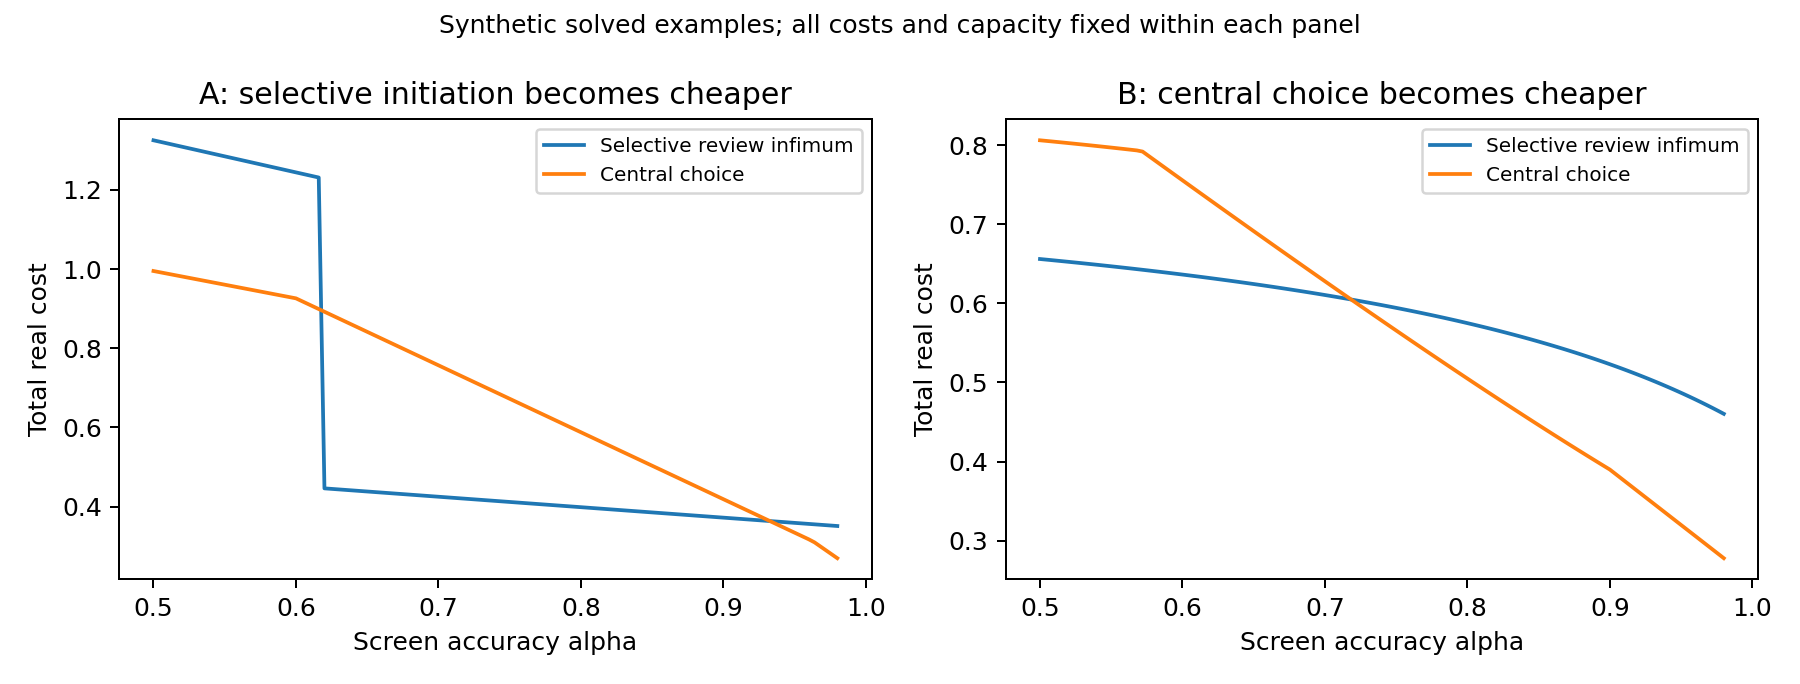
\includegraphics{figures/policy_costs.png}
\caption{Synthetic optimized policy costs. Lines show the solved branch
infimum, which can have threshold discontinuities; they are not
empirical curves.}
\end{figure}

\section{7. Rights and discriminating empirical
measurements}\label{rights-and-discriminating-empirical-measurements}

The model distinguishes the right to initiate, actual filing, central
review, replacement, local final choice and escalation. In S the
initiation right is one; in C it is zero. The filing rate is P=\(\pi+B\)
in S. Testing J is an exercise of a contingent prior veto right;
effective veto/replacement M occurs only when a bad proposal is
detected. Tested proposals that pass are centrally reviewed, not locally
final merely because their action is unchanged.

Two denominators are necessary. Local final positive implementation per
opportunity is \(F_+=P-J\). Local final dispositions including
abstention are \(F_{all}=1-J\) in S, because unsubmitted opportunities
end locally at zero. These are not interchangeable. Conditional rates
among submitted proposals are \(J/P\) and \(M/P\). In C local final
choice is zero by institutional definition, although headquarters may
choose the same action a local manager would have chosen. Escalation to
a third decision maker is absent from this model, so its predicted rate
is zero, not an unidentified relabeling of review.

The new mechanism's discriminating observations are the pre-filing risk
signal and who can see it; the committed test probabilities and actual
compliance; capacity reserved versus tests used; submission and
withdrawal before review; filing effort; test sensitivity and
false-positive performance; and whether lower-temptation opportunities
disappear from the proposal pool. One must record all eligible
opportunities, not just submissions. A fall in replacement with higher
screening precision can reflect deterrence rather than weak monitoring.
Conversely, more corrections do not demonstrate greater local final
authority.

Conditional-MSE first stages remain useful for the original
information-location benchmark in Appendix B. For this binary model the
analogous first stage is calibration and discrimination of
\(P(B\mid s,\mathcal I_0)\) relative to existing information
\(\mathcal I_0\). Verify the improvement among an independently sampled
opportunity set, including unsubmitted cases; observing only tested
proposals creates verification bias. Random validation tests or
authorized external quality outcomes are needed to estimate signal and
detection accuracy. Local private benefits are latent; incentive proxies
do not identify their distribution without further assumptions.

Appendix C retains two feasible modules: an access-by-access experiment
with endogenous authority, and a separate
local-access-by-assigned-authority experiment with central access held
fixed. No experiment has run. Access is not an instrument for authority
because it directly affects performance under fixed authority. A
targeted follow-up could compare two committed screening protocols under
one access rollout, with enough independent approval networks and a
pre-specified first stage. It does not require eight cells, and the
present package promises no field execution.

\section{8. Two opportunities and one non-storable audit
slot}\label{two-opportunities-and-one-non-storable-audit-slot}

\subsection{8.1 A different physical capacity
protocol}\label{a-different-physical-capacity-protocol}

This section replaces neither the population benchmark nor its capacity
definition. A batch contains two independent opportunities, one per
manager. Each is good with probability \(\pi\in(0,1)\) and bad
otherwise. There is one bad benefit b, with \(0<f<b\), and \(V>f\). The
private payoff is \(V-f\) for filing a good project, \(b a-f\) for
filing a bad project implemented with indicator a, and zero for
abstention. The real batch loss is filing effort plus tests plus
bad-implementation harm: \(f E[N_F]+c E[N_T]+H E[N_{BI}]\). Good
projects always file and are never falsely rejected, so their foregone
value is zero in every equilibrium. Private b is not a real resource
loss. Costs f and c are counted once.

Headquarters observes two private binary risk signals, each with
accuracy \(\alpha\in[1/2,1]\), independently conditional on qualities.
Managers know their own quality but observe neither signal, the peer's
type, nor assignment or lottery realizations before simultaneously
filing. Headquarters commits before types. A tested bad filer is
detected with probability \(\zeta\in(0,1]\); no good filer is detected.
Every filed project is implemented unless bad detection occurs. There
are no transfers, penalties beyond rejection, or unverified overrides.
Only one test can occur at every on- and off-path history and every
lottery realization. The slot cannot be stored. Test assignment precedes
any test outcome, so there is no second test after nondetection. The
analysis conditions on this commitment; no new commitment device is
assumed.

We compare two rules on these same primitives and the same physical
slot. A \textbf{fixed assignment} chooses none, manager 1, or manager 2
after both signals but before filings, and wastes the slot if its
recipient abstains. A \textbf{recourse rule} assigns after both signals
and filings, allowing a sole filer to receive the slot. The old
population reservation constraint is neither rule.

Write \(w_B=(\alpha,1-\alpha)\) and \(w_G=(1-\alpha,\alpha)\) for
high/low risk probabilities, and \(m=\pi w_G+(1-\pi)w_B\). A fixed rule
has probabilities \(a_i(s_1,s_2)\geq0\), \(a_1+a_2\leq1\). A recourse
rule has sole-filer probabilities \(u_i(s)\in[0,1]\) and both-filer
probabilities \(v_i(s)\geq0\), \(v_1(s)+v_2(s)\leq1\), at each of four
signal pairs s. With neither filing, no test occurs. These inequalities
are necessary and sufficient for hard feasibility: at each history draw
none or exactly one recipient with the stated probabilities. All
subsequent probabilities refer to such lotteries, never to independent
Bernoulli tests that could exceed capacity.

\subsection{Theorem 6. Complete-deterrence frontiers over all
assignments}\label{theorem-6.-complete-deterrence-frontiers-over-all-assignments}

Let \(t=(1-f/b)/\zeta\). The largest achievable common bad-deviation
test probability, when both bad types abstain and good types file, is

\[Q_F=\tfrac12+\pi(\alpha-\tfrac12)\quad\text{under fixed assignment},\]
\[Q_R=1-\pi+\pi\alpha\quad\text{under recourse}.\]

These maxima hold over arbitrary randomized, asymmetric rules. Complete
bad abstention is a strict BNE if and only if \(t<Q_F\) or \(t<Q_R\),
respectively. Equality permits weak but not strict complete deterrence.
If t exceeds the corresponding maximum, even weak complete deterrence is
impossible. Higher-risk-first assignment with fair ties attains each
frontier; recourse also tests a sole filer with probability one. The
frontier increase is \(Q_R-Q_F=(1-\pi)/2>0\). This is a
target-equilibrium feasibility result, not uniqueness or full
implementation.

\subsection{Theorem 7. Every filing equilibrium, including asymmetry and
equality}\label{theorem-7.-every-filing-equilibrium-including-asymmetry-and-equality}

For a fixed rule define

\[q_{iB}=\sum_s w_B(s_i)m(s_j)a_i(s),\qquad j\ne i.\]

Every BNE is the Cartesian product of the following bad filing
probabilities: \(p_i=0\) if \(q_{iB}>t\), \(p_i=1\) if \(q_{iB}<t\), and
any \(p_i\in[0,1]\) if \(q_{iB}=t\). Good types strictly file.

For an arbitrary recourse rule define

\[A_i=(1-\pi)\sum_s w_B(s_i)w_B(s_j)u_i(s)
 +\pi\sum_s w_B(s_i)w_G(s_j)v_i(s),\]
\[D_i=(1-\pi)\sum_s w_B(s_i)w_B(s_j)[u_i(s)-v_i(s)].\]

A bad deviator's test probability when the peer files with bad-type
probability \(p_j\) is exactly \(A_i-D_i p_j\). The complete BNE set
consists of all \((p_1,p_2)\in[0,1]^2\) satisfying

\[\begin{cases}
 A_i-D_i p_j\geq t,&p_i=0,\\
 A_i-D_i p_j=t,&0<p_i<1,\\
 A_i-D_i p_j\leq t,&p_i=1.
\end{cases}\]

This is an exact nine-support characterization: choose each coordinate's
status from \(\{0,(0,1),1\}\), impose the displayed affine condition on
the other coordinate, and intersect intervals. It covers asymmetric
policies, signed or zero \(D_i\), ties and continua. If both mix and
both \(D_i\ne0\), the only candidate is \(p_1=(A_2-t)/D_2\),
\(p_2=(A_1-t)/D_1\), provided both lie strictly between zero and one.
When \(D_i=0\), its constraint is either vacuous or inconsistent, as
determined by the displayed inequalities, rather than division by zero.

For higher-risk-first recourse, \(A_i=Q_R\) and \(D_i=(1-\pi)/2\). Its
entire equilibrium set is:

\begin{longtable}[]{@{}ll@{}}
\toprule\noalign{}
Threshold & Bad filing probabilities \((p_1,p_2)\) \\
\midrule\noalign{}
\endhead
\bottomrule\noalign{}
\endlastfoot
\(t<Q_F\) & \((0,0)\), strict and unique \\
\(t=Q_F\) & \((0,0)\) strict; \((1,1)\) weak \\
\(Q_F<t<Q_R\) & \((0,0)\) and \((1,1)\) strict; \((p^*,p^*)\) mixed \\
\(t=Q_R\) & \((0,0)\) weak; \((1,1)\) strict \\
\(t>Q_R\) & \((1,1)\), strict and unique \\
\end{longtable}

Here \(p^*=2(Q_R-t)/(1-\pi)\). There are no additional asymmetric
equilibria for this rule, including the two equality cases. Thus
precisely in the open interval where recourse strictly expands the
complete-deterrence target beyond fixed assignment, higher-risk-first
recourse has two strict pure BNE. More screening capacity conditional on
few filings creates strategic complementarity in bad filing, rather than
full implementation.

\subsection{8.2 Exact synthetic witness and an all-rule
obstruction}\label{exact-synthetic-witness-and-an-all-rule-obstruction}

Set \(\pi=\alpha=1/2\), \(\zeta=9/10\), \(b=1\), \(f=2/5\), \(c=1/10\),
\(H=3\), \(V=2\). Then \(t=2/3\), \(Q_F=1/2\), \(Q_R=3/4\). Ignore
signals, audit a sole filer, and choose each with probability 1/2 if
both file. Exact raw-state enumeration gives:

\begin{longtable}[]{@{}
  >{\raggedright\arraybackslash}p{(\columnwidth - 8\tabcolsep) * \real{0.2000}}
  >{\raggedleft\arraybackslash}p{(\columnwidth - 8\tabcolsep) * \real{0.2000}}
  >{\raggedleft\arraybackslash}p{(\columnwidth - 8\tabcolsep) * \real{0.2000}}
  >{\raggedleft\arraybackslash}p{(\columnwidth - 8\tabcolsep) * \real{0.2000}}
  >{\raggedleft\arraybackslash}p{(\columnwidth - 8\tabcolsep) * \real{0.2000}}@{}}
\toprule\noalign{}
\begin{minipage}[b]{\linewidth}\raggedright
Bad filing probability per manager
\end{minipage} & \begin{minipage}[b]{\linewidth}\raggedleft
Expected filings
\end{minipage} & \begin{minipage}[b]{\linewidth}\raggedleft
Expected tests
\end{minipage} & \begin{minipage}[b]{\linewidth}\raggedleft
Bad harm
\end{minipage} & \begin{minipage}[b]{\linewidth}\raggedleft
Total batch loss
\end{minipage} \\
\midrule\noalign{}
\endhead
\bottomrule\noalign{}
\endlastfoot
0 & 1 & \(3/4\) & 0 & \(19/40\) \\
\(1/3\) & \(4/3\) & \(8/9\) & \(2/5\) & \(46/45\) \\
1 & 2 & 1 & \(33/20\) & \(51/20\) \\
\end{longtable}

At the target the bad deviation payoff is \(-3/40\), and a good manager
receives \(8/5\). All three rows are BNE of the same rule and
primitives. These central-review witness values are independently
verified here, not newly discovered empirical or author-origin examples.
The fixed asymmetric rule \(q_1=7/10,q_2=3/10\) has the unique strict
pattern \((0,1)\) and batch loss \(44/25\), smaller than the recourse
both-file loss \(51/20\). The target row does not justify a welfare
recommendation.

\textbf{Theorem 8 (all-rule failure of full implementation at the
witness).} Every hard-feasible recourse rule that supports strict
complete bad deterrence at these primitives also has a strict BNE in
which both bad types file. This holds for asymmetric, randomized,
signal-contingent rules. Therefore no such rule fully implements the
complete-deterrence outcome. It is not merely a defect of
higher-risk-first assignment.

At uninformative signals let \(u_i,v_i\) denote the averages of sole-
and both-filer test probabilities. Strict target deterrence requires
\((u_i+v_i)/2>2/3\). Since \(u_i\leq1\), each \(v_i>1/3\). Hard capacity
gives \(v_1+v_2\leq1\), hence each \(v_i<2/3\). When both bad types
file, everyone always files, so a bad manager is tested with probability
\(v_i<t\) and strictly wants to file. Good filing is always strict. This
proves the obstruction without symmetry or equilibrium selection.

\subsection{Theorem 9. Exact finite-candidate target resource
cost}\label{theorem-9.-exact-finite-candidate-target-resource-cost}

Fix a declared incentive margin \(\eta>0\) in test-probability units and
write \(d=t+\eta\). The target requires \(A_i\geq d\), implying bad
deviation payoff at most \(-b\zeta\eta\). Its resource loss is
\(2\pi f+cT\), where

\[\begin{split}
T=\sum_s\{&\pi(1-\pi)w_G(s_1)w_B(s_2)u_1(s)
+\pi(1-\pi)w_B(s_1)w_G(s_2)u_2(s)\\
&+\pi^2w_G(s_1)w_G(s_2)[v_1(s)+v_2(s)]\}.
\end{split}\]

Enumerate the \(2^8 3^4=20,736\) deterministic hard-feasible policies:
eight sole-filer coordinates are zero or one, and each of four
both-filer histories chooses none, 1 or 2. For policy k compute
\((a_k,T_k)\), where \(a_k=(A_{1k}+A_{2k})/2\). Symmetrize it with its
label-swapped version. The optimal target workload is the lower convex
hull of these projected points evaluated at a=d.~Equivalently, minimize
over vertices with \(a_k=d\) and all pairs with \(a_k<d<a_l\) the finite
list

\[\frac{a_l-d}{a_l-a_k}T_k+\frac{d-a_k}{a_l-a_k}T_l.\]

The problem is feasible exactly when \(d\leq Q_R\). An optimizer uses at
most two symmetrized deterministic policies. This characterization is
constructive, accounts for each signal/filing history, and is
independently checked against a 16-variable raw-probability linear
program. Symmetrization here preserves convex target IC and the linear
target objective; it says nothing about preserving all equilibria or
worst-equilibrium welfare.

At the uninformative witness, every symmetrized target policy has
\(T=A=(A_1+A_2)/2\). Thus

\[L_{R,\mathrm{target}}(d)=\frac25+\frac{d}{10},\qquad 0<d\leq\frac34.\]

For strict deterrence with no fixed positive margin the loss infimum is
\(7/15\), not attained because \(d=2/3\) only gives weak target IC. For
a declared \(\eta\in(0,1/12]\) the attained minimum is \(7/15+\eta/10\).
For example \(\eta=1/60\) gives \(d=41/60\), loss \(281/600\), and can
be implemented by testing a sole filer with probability one and each
both-filer with probability \(11/30\). This cost-minimizing target
policy still has a strict both-file BNE by Theorem 8 (its additional
symmetric mixed BNE has bad filing probability \(1/19\)). Its low target
cost is not its robust governance value.

\subsection{8.3 Best fixed assignment and an informative-signal
region}\label{best-fixed-assignment-and-an-informative-signal-region}

\textbf{Proposition 10 (fixed-assignment comparison at the witness).}
Over all fixed rules and all their BNE, the smallest achievable loss is
\(103/60\) if favorable mixing at an indifferent bad type is allowed. It
is attained at \(q_1=2/3,q_2=1/3\), with the first bad type abstaining.
Among rules with strict bad-type responses, \(103/60\) is only an
infimum. With a declared distance \(\eta\in(0,1/6]\) from the threshold
for both responses, the attained minimum is \(103/60+13\eta/10\). At
\(\eta=1/30\) it is \(44/25\), implemented by the asymmetric rule above.
The all-file region has minimum \(51/20\). Indifferent first-manager
mixing is explicitly included, not silently assigned a favorable tie.

For the same \(\pi,\zeta,b,f,c,H,V\), but \(\alpha\in[1/2,5/6)\), every
fixed rule and every BNE has bad harm alone bounded below by

\[\frac{69}{40}-\frac{27}{20}\alpha>\frac35>\frac{19}{40}.\]

The risk-ignoring recourse target with loss \(19/40\) remains feasible
and strict throughout this interval, including the informative
subinterval \((1/2,5/6)\). Consequently its target cost is below every
fixed-rule equilibrium cost there. This is a target comparison, not a
comparison of worst equilibria: the recourse rule also retains its bad
equilibrium. The endpoint \(5/6\) is excluded because both
fixed-assignment bad types can then be indifferent and abstain weakly.

\subsection{8.4 Rights, measurement and bounded
interpretation}\label{rights-measurement-and-bounded-interpretation}

Both rules formally allow either manager to initiate. Their distinction
is the timing of slot assignment and contingent redeployment, not a
newly defined authority right. In the target only good managers file,
nobody is replaced, and managers retain the final abstention decision on
bad opportunities. In the both-file equilibrium initiative is more
frequent and bad detection creates more central replacement. The same
formal rights and screen accuracy can therefore produce very different
observed initiative and intervention. Conditional-MSE measures in
Section 7 remain first stages for information quality, not instruments
for authority.

The discriminating operational measurement is the assignment probability
conditional on both risk scores and the complete filing profile,
especially the change from both filers to a sole filer. Record
preassignment timestamps, unused slots, final recipient, test outcomes,
filed and unfiled opportunities, and repeated batches. A low target
workload with few bad filings does not establish that deviations would
receive timely tests, or rule out another equilibrium. This suggests a
modest protocol measuring recourse and filing responses rather than an
infeasible eight-cell study. No such study has been run.

\section{9. Conclusion}\label{limitations-and-conclusion}

The population benchmark solves reserved service capacity and
heterogeneous bad temptations; the finite-batch extension solves two
independent opportunities and one hard slot. They are distinct
institutions. Neither solves general queues, optimal information
acquisition, noncommitted review, multidimensional reporting or a
general organizational optimum. The recourse cost result optimizes a
declared target with positive IC margin; it is not a worst-equilibrium
optimization. The uninformative all-rule obstruction establishes failure
of full implementation of complete deterrence, not impossibility of
every useful recourse policy or a global welfare ranking.

Better central access can alter initiative and intervention, but
contingent review capacity also creates endogenous congestion and
equilibrium multiplicity. The finite frontier is achievable; the
favorable outcome need not be unique. Remaining material objections are
the narrow primitives and commitment assumption, limited novelty
relative to existing verification theory, and an incomplete
theorem-level comparison to Habermacher's final article. No firm data,
empirical estimates or field evidence are supplied. Appendix C is
prospective. These are completed bounded mathematical results with
reproducible synthetic checks, not evidence of practical effectiveness
or a claim of publication readiness.


{
\small
\setlength{\parindent}{0pt}
\section*{References}\label{references}

Aghion, Philippe, and Jean Tirole. 1997. ``Formal and Real Authority in
Organizations.'' \emph{Journal of Political Economy} 105(1): 1-29.
\url{https://doi.org/10.1086/262063}.

Alonso, Ricardo, Wouter Dessein, and Niko Matouschek. 2008. ``When Does
Coordination Require Centralization?'' \emph{American Economic Review}
98(1): 145-179. \url{https://doi.org/10.1257/aer.98.1.145}. Corrigendum:
\emph{American Economic Review} 98(3): 1195-1196.
\url{https://doi.org/10.1257/aer.98.3.1195}.

Argenziano, Rossella, Sergei Severinov, and Francesco Squintani. 2016.
``Strategic Information Acquisition and Transmission.'' \emph{American
Economic Journal: Microeconomics} 8(3): 119-155.
\url{https://doi.org/10.1257/mic.20140135}. Inspected author version: final
submission, November 2015.

Bloom, Nicholas, Luis Garicano, Raffaella Sadun, and John Van Reenen.
2014. ``The Distinct Effects of Information Technology and Communication
Technology on Firm Organization.'' \emph{Management Science} 60(12):
2859-2885. \url{https://doi.org/10.1287/mnsc.2014.2013}.

Erlanson, Albin, and Andreas Kleiner. 2024. ``Optimal Allocations with
Capacity Constrained Verification.'' arXiv:2409.02031.
\url{https://doi.org/10.48550/arXiv.2409.02031}. Working paper; retrieved HTML
body dated August 24, 2026, although landing-page submission history
lists September 3, 2024.

Habermacher, Daniel. 2025. ``Authority and Specialization Under
Informational Interdependence.'' \emph{RAND Journal of Economics} 56(4):
562-586. \url{https://doi.org/10.1111/1756-2171.70021}. Published
metadata/abstract verified; final full text unavailable. Separately
inspected earlier version: RedNIE Working Paper 142, May 5, 2022,
\url{https://rednie.eco.unc.edu.ar/files/DT/142.pdf}.

Halac, Marina, and Pierre Yared. 2020. ``Commitment versus Flexibility
with Costly Verification.'' \emph{Journal of Political Economy} 128(12):
4523-4573. \url{https://doi.org/10.1086/710560}. Final published author-hosted
PDF inspected; not confused with NBER Working Paper 22936 or its 2017
revision.

Labro, Eva, Mark Lang, and James D. Omartian. 2023. ``Predictive
Analytics and Centralization of Authority.'' \emph{Journal of Accounting
and Economics} 75(1): 101526.
\url{https://doi.org/10.1016/j.jacceco.2022.101526}.

Wu, Lynn, Bowen Lou, and Lorin Hitt. 2019. ``Data Analytics Supports
Decentralized Innovation.'' \emph{Management Science} 65(10): 4863-4877.
\url{https://doi.org/10.1287/mnsc.2019.3344}.

}
\clearpage
\section{Appendix A. Complete proofs and implementation
details}\label{appendix-a.-complete-proofs-and-implementation-details}

\subsection{A1. Proof of Theorem 1 and all
deviations}\label{a1.-proof-of-theorem-1-and-all-deviations}

In S, m=0 guarantees a=0 at zero filing cost for every type. A good
proposal is never rejected: neither a negative test nor a test of a good
opportunity triggers detection. Therefore the net gain from m=1 over m=0
is V-f\textgreater0 for G. For Bi, implementation probability
conditional on s is \(1-\zeta q_s\). Averaging over its private
pre-filing information, the gain is \(b_i(1-\zeta Q_B)-f\). Comparing
this single deviation with zero gives the full best-response
correspondence. No other messages or actions are available. Mixed
strategies can be optimal only at equality; any mixing probability then
yields the same manager payoff.

Bad classes have identical conditional signal distributions. Hence the
aggregate submitted bad mass B is independent of s conditional on bad
quality. Bayes' rule gives the posterior in Theorem 1. At a
zero-probability abstention history, the committed default remains zero;
G cannot gain by creating it. At a zero-probability bad submission, the
announced signal-conditioned test remains feasible by the all-submission
reservation constraint and yields the deviation payoff already checked.
The principal's committed continuation does not require a
belief-dependent optimality condition. Without commitment this is a
different game, addressed only in Proposition 4(c).

All good opportunities are implemented, so no missed-good loss occurs in
S. The mass of filings is \(\pi+B\), tests J, and undetected implemented
bad opportunities \(B(1-\zeta Q_B)\). Multiplying by f,c,H respectively
and summing proves (2). Increasing a threshold type's participation
raises cost by its population mass times \(f+cQ_B+H(1-\zeta Q_B)>0\).
Thus worst-equilibrium selection at indifference is filing. Formula (2)
also proves all rights rates stated in Section 7.

\subsection{A2. Proof of Theorem 2}\label{a2.-proof-of-theorem-2}

For \(\alpha>1/2\), eliminate \(q_L\) from the constraint
\(\alpha q_H+(1-\alpha)q_L=Q\). Good scrutiny becomes

\[Q_G=\frac{\alpha Q}{1-\alpha}+\frac{1-2\alpha}{1-\alpha}q_H.\]

The coefficient of \(q_H\) is negative. Therefore minimize \(Q_G\) by
maximizing \(q_H\), subject to \(0\leq q_H,q_L\leq1\). If
\(Q\leq\alpha\), this gives \(q_H=Q/\alpha,q_L=0\); if \(Q\geq\alpha\),
it gives \(q_H=1,q_L=(Q-\alpha)/(1-\alpha)\). Substitution yields (3).
For \(\alpha=1/2\), both conditional probabilities equal
\((q_H+q_L)/2\), giving the same value.

At fixed Q and submission mass B, cost (2) depends positively on \(Q_G\)
through \(c\pi Q_G\). Reservation depends positively on \(Q_G\) through
\(\pi Q_G\). Thus the frontier weakly dominates every other rule with
the same Q, and the domination in cost is strict off the frontier for
\(c\pi>0\). This proves the optimality reduction without presuming that
proposals are truthful.

The function \(\kappa_\alpha(Q)\) is continuous and strictly increasing
from zero to one because \(\pi\in(0,1)\) and \(\gamma\) is increasing.
Strict deterrence needs \(Q>t_i\). Such Q is feasible exactly when
\(t_i<1\) and \(K>\kappa_\alpha(t_i)\). Equality in capacity only
permits weak indifference. Solving \(\kappa_\alpha(Q)=K\) on its two
linear segments gives (5), since \(\kappa_\alpha(\alpha)=m_H\).

Fix Q while varying accuracy \(\alpha\). On the region \(\alpha>Q\),
\(\partial\gamma_\alpha(Q)/\partial\alpha=-Q/\alpha^2<0\). On the region
\(\alpha<Q\), write
\(\gamma_\alpha(Q)=(1-2\alpha+\alpha Q)/(1-\alpha)\), whose derivative
is \((Q-1)/(1-\alpha)^2<0\) for Q\textless1. For a fixed
\(Q\in(1/2,1)\), the two regions meet at the admissible interior point
\(\alpha=Q\). Both values there are \(1-Q\), but the one-sided accuracy
derivatives are

\[\left.\partial_\alpha^-\gamma_\alpha(Q)\right|_{\alpha=Q}=-\frac{1}{1-Q},\qquad
\left.\partial_\alpha^+\gamma_\alpha(Q)\right|_{\alpha=Q}=-\frac{1}{Q}. \tag{9}\]

They are unequal for every interior crossing Q\textgreater1/2. At Q=0.7
the values are \(-10/3\) and \(-10/7\). The algebraic expressions agree
only at Q=1/2, where the crossing is a boundary of the admissible
accuracy domain and only the right derivative is required. For
Q\textless1/2 there is no interior crossing in \(\alpha\in[1/2,1)\). For
Q=0 and Q=1 the frontier is constant in accuracy.

Thus the frontier is continuous and piecewise differentiable, not
continuously differentiable across the interior crossing. For any two
accuracies and fixed Q in (0,1), it strictly decreases on each nonempty
piece between them. If their interval straddles Q, split it at Q and use
continuity plus strict decrease on the two pieces. This proves strict
decrease on the whole interval without assuming a common derivative.
Since \(\kappa_\alpha(Q)=\pi\gamma_\alpha(Q)+(1-\pi)Q\) and \(\pi>0\),
the same strict decrease holds for (4); its one-sided accuracy
derivatives are \(-\pi/(1-Q)\) and \(-\pi/Q\) at an interior crossing.
Theorem 2 therefore survives the correction.

For clarity, differentiating with respect to Q at fixed accuracy is a
different calculation: the slopes on the two sides of Q=\(\alpha\) are
\((1-\alpha)/\alpha\) and \(\alpha/(1-\alpha)\). These are both positive
and need not agree either. Theorem 3 uses their piecewise affine form
and the kink as a candidate, not differentiability at that point.

\subsection{A3. Proof of Theorem 3, tie boundaries and
attainment}\label{a3.-proof-of-theorem-3-tie-boundaries-and-attainment}

Theorem 1 and \(t_1<t_2\) imply that the only strict participation
patterns are both bad types file, only B2 files, and neither files. At
\(Q=t_1\) worst selection includes B1; at \(Q=t_2\) it includes B2.
These yield exactly the actual branch domains stated. Thresholds above
one are unreachable. The attainable set of Q is \([0,\bar Q]\) by A2. A
right-hand branch whose lower endpoint cannot be crossed has no actual
points and cannot contribute a one-sided value to the optimization.

Substitute B=\(B_j\) and the frontier \(Q_G=\gamma_\alpha(Q)\) into (2)
to obtain (6). On every segment on which \(\gamma\) is affine,
\(\ell_j\) is affine. A linear function on an interval takes its minimum
at an endpoint, unless constant, in which case every point is
minimizing. Therefore its infimum on a possibly half-open branch is
obtained by evaluating its closure endpoints and its one kink, if
included. Taking the minimum across finitely many branches proves the
value formula.

An attained global minimum must lie in an actual branch and equal that
value. Conversely, any minimizing point in an actual branch implements
the value, by the frontier rule and worst-equilibrium participation. If
no minimizing point belongs to an actual branch, minima of the closures
occur only at excluded lower endpoints. Since each such branch has
actual points, a sequence from its right approaches the boundary with
the same participation and continuous within-branch cost. This proves
the existence of arbitrarily close strictly deterrent policies, but not
an optimal policy at the boundary. At an upper threshold, worst
selection is the branch's still-active type, so that endpoint is
included. If a minimizing face contains an included point, the value is
attained even if one minimizing endpoint is excluded.

With the \(\eta\) restriction each nonempty interval is compact. The
same argument yields an attained minimum. Finite-type indifference is
not used to select favorable behavior. This construction also clarifies
that a closed-branch linear program must check branch nonemptiness
before counting a deterrent boundary solution.

\subsection{A4. Proof of central-choice formula and D
optimality}\label{a4.-proof-of-central-choice-formula-and-d-optimality}

Under C, at signal s, accepting gives unconditional error cost \(b_sH\)
and rejecting gives \(g_sV\). A test detects B with unconditional
probability \(\zeta b_s\), in which case rejecting is optimal. Following
no detection, the remaining unconditional good and bad masses are
\(g_s\) and \((1-\zeta)b_s\). Correct Bayesian choice therefore
contributes \(\min\{g_sV,(1-\zeta)b_sH\}\); the test cost is \(cm_s\).
This yields \(a_s\) and (7).

A randomized test at s averages the tested and untested costs linearly.
To minimize cost under \(\sum m_sr_s\leq K\), consider two signals i,j
with net benefit per slot at i greater than at j. If j receives a
positive test share while i is not saturated, move an equal mass of
slots from j to i. Feasibility is unchanged and total cost falls.
Therefore all profitable signals are tested in descending
benefit-per-slot order, and none with negative gain is tested unless
indifferent. This proves optimality including fractional capacity
boundaries. Overhead d is added once per opportunity, and not charged
again as a test cost.

In the unreviewed binary delegation class, prohibiting positive action
gives D0. Allowing it makes every type strictly prefer filing and
implementation, since V and both b values exceed f.~There is no other
nonempty voluntary binary delegation set beyond a standing prohibition
or permission to implement. The loss of D1 is filing f for every
opportunity plus bad implementation loss \((1-\pi)H\). Their minimum is
optimal in that class. Forced implementation and rich message mechanisms
are not part of this delegation definition.

\subsection{A5. Proof of Proposition
4}\label{a5.-proof-of-proposition-4}

\begin{enumerate}
\def\labelenumi{(\alph{enumi})}
\item
  With f=0, strict deterrence requires \(b_i(1-\zeta Q_B)<0\),
  impossible because \(\zeta Q_B\leq1\). Even weak indifference needs
  \(\zeta Q_B=1\). If \(\zeta<1\), this is impossible. If \(\zeta=1\)
  and \(\alpha<1\), both conditional signal probabilities are positive,
  so \(Q_B=1\) forces \(q_H=q_L=1\). Then reservation is one, infeasible
  at K\textless1. Thus bad types strictly file under scarce capacity.
  Positive f opens an interval in which not filing is strictly better,
  but it does not guarantee feasibility; Theorem 2 gives the threshold.
\item
  With one bad benefit and off its threshold, the best response is all
  file or all abstain. In any deterrent branch B=0, so
  \(M=\zeta BQ_B=0\). There is no unique-equilibrium partial
  participation. Heterogeneity permits a strictly deterred class and a
  strictly participating class at the same Q, as the example verifies.
  This establishes necessity within the homogeneous baseline, not a
  unique minimal friction across all possible games.
\item
  If all bad managers abstain, an on-path positive proposal is known
  good. A test cannot change its optimal action and costs
  c\textgreater0. A center free to revise its plan therefore chooses
  zero testing on every on-path signal. A bad manager then obtains
  \(b_i-f>0\) by proposing. This contradicts complete deterrence.
  Committed testing is not a sequential best response in that history;
  it is an institutional restriction imposed ex ante. The proof does not
  assert a full characterization of the no-commitment game.
\item
  For any S mechanism and its equilibrium, a center possessing the same
  message, commitment and testing technology can select the identical
  map from messages, signals and test outcomes into actions. Its
  equilibrium incentives, costs and capacity use are then identical. A
  feasible set that includes this map has optimum weakly better. Strict
  S dominance is impossible without an additional feasible-set or
  real-cost distinction. This is a replication argument, not a new
  delegation theorem.
\end{enumerate}

\subsection{A6. Proof of Proposition 5 and the
examples}\label{a6.-proof-of-proposition-5-and-the-examples}

Let \(\alpha'>\alpha\geq1/2\). Generate the old signal from the new one
by independently flipping it with probability
\(r=(\alpha'-\alpha)/(2\alpha'-1)\in[0,1/2]\). The resulting signal has
conditional accuracy \(\alpha'-(2\alpha'-1)r=\alpha\). A center can
apply the old rule to this garbled signal. Under S, both \(Q_G\) and
\(Q_B\) are unchanged, hence participation, reservation, costs and
worst-equilibrium outcomes are unchanged. Under C, the center can also
reproduce its original signal/test/decision process. Optimization over
the richer feasible choices cannot increase either value. The degenerate
case \(\alpha=\alpha'=1/2\) is immediate.

On a high-risk-only capacity segment, \(Q_B=\alpha K/m_H\) and
\(Q_G=(1-\alpha)K/m_H\), with \(m_H=\pi+(1-2\pi)\alpha\). Quotient
differentiation yields (8). Replacement is \(\zeta BQ_B\) at fixed B,
and can jump down when participation falls. There is no derivative claim
across that jump.

For both examples, the closed-branch vertices and the frontier endpoints
give \(q_H=K/m_H\), \(q_L=0\) as the unique selective optimum. In
Example A, mH=0.5 at both accuracies, so qH=0.6. At low accuracy
\(\bar Q=0.33<t_1\); there is only the pooling branch. At high accuracy
\(\bar Q=0.54<t_2\); direct evaluation of the pooling closure gives a
minimum 1.220576, while the B1-deterrent branch gives 0.3724. Its
within-first-frontier-segment slope is
\(0.1\cdot0.5(0.1/0.9)+(0.1-2.7)\cdot0.15<0\), so its optimum is the
capacity endpoint. All incentive inequalities there are strict. Applying
(7) yields C values 0.9605 and 0.4190. Comparing with D0=1 and D1=1.7
proves the strict C-to-S switch. Rights and cost numbers follow from
(2).

For Example B, \(t_1=1\) and \(t_2>1\), so only pooling is feasible. At
low accuracy mH=0.47 and qH=10/47; at high accuracy mH=0.23 and
qH=10/23. The pooling cost slope is negative until capacity is
exhausted; these endpoints are optimal. Formula (7), including
negative-test updating, gives central costs 0.7968085 and 0.32. D0=0.8
and D1=0.7 complete the strict S-to-C comparison. The cost gaps are
nonzero, the incentive constraints strict and the capacity endpoints
below qH=1. These properties persist in a neighborhood of the displayed
primitives, so the switches are not indifference artifacts.

\subsection{A7. Independent verification and boundary
cases}\label{a7.-independent-verification-and-boundary-cases}

The reproduction code uses three formulations of the selective problem:
scalar frontier evaluation, intersections of the seven two-dimensional
branch boundaries, and HiGHS linear programming. The central benchmark
is checked both by its geometric two-dimensional review problem and by a
six-variable action/test linear program. A separate enumerator sums
type, signal, test and detection events and recomputes manager deviation
payoffs without using the cost formula. These checks agree for the two
examples and for 160 additional parameter configurations. A separate
standard-library-only rational-arithmetic program certifies all four
example optima and governance rankings exactly, without NumPy, SciPy or
floating-point arithmetic. The latter are implementation checks, not
evidence of economic relevance.

R2 adds deterministic exact-rational one-sided difference-quotient
checks at the accuracy kink, including Q=0.7, and a check of the
reservation/workload gap. The existing optimization examples and their
certificates remain unchanged. Boundary checks include zero capacity;
zero detection; an uninformative signal; free proposals; threshold
indifference; and capacity exactly equal to a deterrence requirement.
The last case must not be counted as strict deterrence. A dense
audit-probability grid supplies an additional upper-bound check, but is
not the optimization proof. Computations use Python because Rscript was
unavailable on the session PATH; editable LaTeX and all algorithms are
supplied.

\section{Appendix B. Information-location benchmark, explicitly
non-novel}\label{appendix-b.-information-location-benchmark-explicitly-non-novel}

For \(L(a)=(a-x)^2+k(a-g)^2\), a local manager knows x and a posterior
mean \(m_L\) for g, with conditional MSE v, and has local target bias b.
The center knows g and posterior mean \(m_C\) for x, with conditional
MSE u. Under a restricted no-free-message comparison,

\[a_D=(x+b+km_L)/(1+k),\quad a_C=(m_C+kg)/(1+k).\]

Completing the square at \(a^*=(x+kg)/(1+k)\) gives excess loss
\((1+k)(a-a^*)^2\). Posterior-mean orthogonality then gives
\(R_D=(b^2+k^2v)/(1+k)\) and \(R_C=u/(1+k)+d\). Therefore D weakly
dominates C exactly when \(u-b^2-k^2v+(1+k)d\geq0\). The derivation is
elementary and does not constitute the new result.

A local improvement \(\delta_v\) lowers delegated loss by
\(k^2\delta_v/(1+k)\); a central improvement \(\delta_u\) lowers central
loss by \(\delta_u/(1+k)\). These zero cross-regime effects are
consequences of the information assignment. They are not universal
treatment interactions. With gains depending on k, the local derivative
adds \(k^2\delta_v'(k)/(1+k)\), which can overturn the sign. With
correlated states, posterior means and MSEs must condition on the
recipient's entire existing information. With a biased deployed
forecast, the cross term \(2bkE[m_L-g]\) need not vanish. This appendix
motivates conditional-MSE first stages in Appendix C and makes no
strategic-screening inference.

\section{Appendix C. Prospective empirical
protocol}\label{appendix-c.-prospective-empirical-protocol}

The full protocol below is unrun. It is also supplied separately as
\path{appendices/Field_Protocol.md}. Its baseline modules are
retained, while the R1 addendum identifies measurements for the new
strategic-screening mechanism.

\subsection{Pre-results empirical
protocol}\label{pre-results-empirical-protocol}

Paper 06. Revision R3, 17 October 2026. No registration or experiment
has occurred. This is a proposed protocol requiring a partner-specific
feasibility amendment before assignment. Analysis unit and estimands
precede method selection.

\subsubsection{R1 mechanism-specific addendum: not yet
implemented}\label{r1-mechanism-specific-addendum-not-yet-implemented}

This addendum supplements the existing two modules without adding an
eight-cell experiment. The new theoretical model concerns central
screening and strategic submission; the previous local-information
interaction remains a separate benchmark. Neither has been tested in
firms.

Record a pre-treatment inventory of all eligible opportunities,
including those never submitted. Log the risk statistic available before
filing, whether local staff could observe it, the published test
probabilities, randomization draws, reserved review slots, actual slots
used, test completion and detection outcomes, and every action
replacement. Record proposal preparation time and central processing
time separately. A negative test is not a verified good project.
Estimate sensitivity and false positives using authorized validation
outcomes or a random validation sample across submitted and unsubmitted
opportunities; selectively tested proposals alone do not identify
accuracy.

Preserve these distinct endpoints: initiation rights; actual filing per
opportunity; effective local abstention; unreviewed positive
implementation F\_plus; all local final dispositions including
abstention F\_all; central review J; central replacement M; and
escalation to a third decision maker. Test M/P and J/P only alongside
unconditional opportunity-denominator rates. In the model F\_plus=P-J
and F\_all=1-J, while escalation is zero. These identities are coding
checks, not assumed data facts. Passing a reviewed proposal unchanged
does not create local final authority.

The model predicts a threshold response in filing composition when
conditional scrutiny crosses a temptation-specific incentive threshold.
Distinguishing it requires measured filing costs and independently
assessed quality among nonfilers; latent private benefits are not
observed or identified by a dashboard log. Observing fewer bad
submissions after access is consistent with deterrence but also with
selection, reclassification or new opportunities. Record these
alternatives. A conditional risk/MSE first stage must assess new
information relative to prior recipient knowledge, before the proposal
response changes the tested sample.

A feasible next study might vary a committed screening rule within a
single access programme, holding authority envelopes and safety
protections fixed, if enough independent networks exist. It would
require a new, powered protocol and authorization. No such intervention,
partner, random assignment or protocol registration is claimed. Existing
Studies A and B below remain separate proposals. Access must not
instrument authority: its direct performance effects violate the
exclusion restriction.

\subsubsection{R3 finite-batch measurement addendum: prospective
only}\label{r3-finite-batch-measurement-addendum-prospective-only}

Before any intervention, establish whether slots are assigned before
filing or can move after abstention. Log both risk scores, assignment
timestamps, the complete filing profile, sole-filer and both-filer audit
probabilities, unused slots and the realized test recipient. Distinguish
rejection after detection from locally chosen abstention. Small
repeated-batch observations may identify congestion patterns but do not
identify an equilibrium-selection effect without additional assumptions.
Conditional-MSE validation of information access remains separate.
Access is not an instrument for authority. No eight-cell study is
promised, no recruitment or intervention has occurred, and no empirical
result is reported.

\subsubsection{1. Setting, units and
eligibility}\label{setting-units-and-eligibility}

Choose one repeated, low-risk operational decision class with a
predetermined firm-wide capacity or coordination target. Candidate:
replenishment within an approved quantity range. No company or dataset
is asserted to exist. Exclude safety-critical decisions, regulated
approval requirements, employment actions, decisions outside the budget
envelope and opportunities without a locked pre-decision benchmark.

An opportunity enters the denominator when the operating system first
generates an eligible need, before anyone chooses whether to act.
Include inaction, cancellation, abandonment and escalation. A
post-treatment sample consisting only of implemented decisions is
unacceptable. Primary outcome is defined for every opportunity over a
fixed 30-day window; a partner-specific alternative must be locked
before randomization.

The assignment unit is an approval network: local units sharing an
approver, capacity constraint or frequently exchanged information.
Cluster across connected units where possible. If headquarters is one
indivisible network, repeated decisions do not supply independent
central-access assignments. Study A is infeasible as a cluster RCT in
that firm; use multiple independent networks or retain a descriptive
case study. Cluster size and network count, not clicks or rows,
determine precision.

\subsubsection{2. Interventions}\label{interventions}

Central access C: verified, new local-state information available to the
central approver. Local access L: verified, new shared-constraint
information available to the local decision maker. Keep interface,
training time, messaging functionality, alerts and approval latency as
similar as possible. The control retains all existing access. Never
remove safety-critical information. Treatment adds access to relevant
noncritical information rather than permission to ignore required
controls.

D=1: local final authority within the eligible envelope, with no routine
prior central approval. D=0: central final authority under the usual
deadline. Mandatory exception routes remain in both arms and are logged.
Consultation is permitted but recorded. A D arm with routine informal
prior approval is noncompliance, not true delegated authority.

A selective-review intervention is outside these baseline confirmatory
modules. The new model motivates measurement of committed risk-based
testing, not an uncosted fourth randomized factor. A separate protocol
would be required to vary screening rules.

\subsubsection{3. Studies and causal
estimands}\label{studies-and-causal-estimands}

Study A is a balanced 2x2 C-by-L cluster experiment under existing
authority arrangements. A(c,l) is the indicator of local final choice
without prior central approval. Y(c,l) is negative total opportunity
cost. Primary family: marginal ITT of C on A and marginal ITT of L on A,
each averaging equally over the other assigned factor. Use Holm
correction across these two tests at familywise 5 percent. Performance
and C-by-L interaction are secondary unless powered and promoted before
assignment. They are effects of access with endogenous organizational
response.

Study B is a separate balanced 2x2 L-by-D experiment, with central
access fixed. Primary contrast: E{[}Y(1,1)-Y(0,1)-Y(1,0)+Y(0,0){]}, with
notation (L,D). This is a single two-sided confirmatory test at 5
percent. D effects and L effects are secondary. The pre-designated
heterogeneity question is whether the L-by-D contrast rises with
baseline coordination exposure K. It remains exploratory unless blinded
pilot-based power supports it and a revised protocol explicitly promotes
it before treatment assignment.

Separate sites or nonoverlapping cohorts avoid carrying learning and
access from A to B. If sequential use of the same networks is
unavoidable, the second study targets incremental effects conditional on
prior history, not a fresh untreated factorial. No washout of knowledge
is presumed.

There is no instrument for actual authority in Study A. Access directly
affects Y, violating the exclusion restriction that would usually be
needed to instrument authority with access. ITT of assigned D in Study B
remains interpretable under noncompliance. A complier authority effect
is not primary and requires additional exclusion, monotonicity and
interference assumptions that may fail through approval delays or
expectations.

\subsubsection{4. Outcomes and economic
interpretation}\label{outcomes-and-economic-interpretation}

Primary Study B cost includes direct operating cost, shortage or rework
cost, a pre-agreed shadow price for capacity deviations, staff review
time and delay cost. Define the accounting map using historical cost
systems before assignment. Subtracting it defines Y so higher is better.
Use ledger-based components and a transparent sensitivity range for
shadow prices. Do not tune weights to favor delegation. A smaller
own-unit cost with larger losses elsewhere is not a success.

Primary Study A authority endpoint is binary local final choice without
prior central approval. Parallel secondary endpoints: local initiation,
central revision, successful veto, escalation, implementation time,
approval waiting time, staff time and coordination deviation. Label
elapsed time versus monetized delay clearly to avoid charging the same
delay twice. Satisfaction and perceived autonomy are exploratory.

Minimum economically meaningful effect for Study B: a partner-agreed 5
percent reduction in historical mean total cost, including all
opportunities. That threshold is a design choice, not a claimed
universal business standard. Convert it to SD units using a blinded
pilot. For Study A, a 10 percentage point change in local final choice
is the provisional planning target. Binary endpoint precision depends on
baseline prevalence and clustering; the standardized table below is not
a binary power calculation.

\subsubsection{5. Measurement and validation
plan}\label{measurement-and-validation-plan}

Permissions, content quality, use and rights are separate fields.
Compare information against what the recipient already knew at baseline.
Pre-decision forecast tasks elicit local estimates of shared constraints
and central estimates of local conditions, using consistently timed
questions in all arms. Forecast error gives a first stage closer to u
and v; access logs alone do not. Elicitation itself may alter use, so
keep it identical across arms and test operational burden in a pilot.

Draw an arm-stratified sample of at least 10 percent of opportunities,
minimum 50 per cell if available, for double coding by reviewers blinded
to performance. Code event order, substantive revisions and whether
approval preceded implementation. Pre-specify at least 90 percent raw
agreement as a provisional go/no-go criterion; report chance-adjusted
agreement and a confusion matrix. Failure triggers instrument repair
before the confirmatory study. These thresholds are planning
assumptions, not completed validation results.

Reconcile every implemented action with an opportunity ID. Report
unmatched actions and opportunities. Distinguish a recommendation
adopted unchanged from a nominal local approval of a central choice.
Brief confidential process interviews, only if separately authorized,
may detect off-system influence; none have been conducted or arranged.

\subsubsection{6. Assignment and
inference}\label{assignment-and-inference}

Within baseline strata defined by network size, task family and baseline
coordination exposure, randomize clusters equally to four cells using a
recorded seed. Obtain enough strata to preserve balance without
singleton cells. Allocation is executed only after eligibility and
baseline data are frozen. No randomization has been performed in this
package.

Estimate a saturated factorial model of Y on L, D and LD plus
randomization-stratum indicators and pre-specified baseline outcome
covariates. With 0/1 coding the LD coefficient estimates the
interaction. For marginal main effects average the relevant cell means
explicitly; do not mistake a conditional coefficient for the marginal
effect. Report cell means and contrasts with confidence intervals.

Use assignment-network clustered standard errors and randomization
inference respecting strata; with few clusters prioritize exact or Monte
Carlo assignment-based inference and disclose attainable p-value
resolution. Evaluate equal-network-weight and opportunity-weight
estimands separately. The primary estimand is opportunity-weighted over
baseline eligible volume, using fixed baseline weights so
treatment-induced volume does not change the target population.
Pre-specify these weights before assignment. Report an
equal-network-weight sensitivity analysis.

\subsubsection{7. Precision and feasible
scope}\label{precision-and-feasible-scope}

Illustrative assumptions only: equal cell sizes; J independent clusters;
40 opportunities per cluster; ICC 0.10; standardized opportunity outcome
variance 1; no baseline variance reduction; two-sided 5 percent and 80
percent power under a normal approximation. Effective sample size is
N\_eff=40J/{[}1+39(0.10){]}. Approximate MDE for a factorial marginal
main effect is 2.8\emph{2/sqrt(N\_eff), and for a
difference-in-differences interaction 2.8}4/sqrt(N\_eff).

\begin{longtable}[]{@{}rrr@{}}
\toprule\noalign{}
Independent clusters & Main-effect MDE, SD & Interaction MDE, SD \\
\midrule\noalign{}
\endhead
\bottomrule\noalign{}
\endlastfoot
80 & 0.219 & 0.438 \\
160 & 0.155 & 0.310 \\
320 & 0.110 & 0.219 \\
640 & 0.077 & 0.155 \\
\end{longtable}

Thus 80 clusters cannot credibly detect a 0.15 SD interaction under
these assumptions. A 0.20 SD interaction requires approximately 385
clusters before accounting for imbalance, small-sample inference or
multiplicity. This is a warning against an eight-cell study and strong
heterogeneity claims. No sample size has been secured. Simulate power
using the actual baseline network, skewness, missingness and assignment
strata before launching; the analytic table is only a screening
calculation.

\subsubsection{8. Identification assumptions and
threats}\label{identification-assumptions-and-threats}

Random assignment identifies assignment effects if allocation is
implemented as designed, outcomes have consistent definitions,
eligibility is fixed before exposure and exposure across networks is
negligible or modeled. Sharing a dashboard, moving staff, or a common
approver contaminates arms. Measure cross-network links and report
treatment exposure of neighbors. If residual interference is
substantial, estimate network-level total effects or specify a two-stage
saturation design in a new protocol. Do not relabel an individual direct
effect as a firm-wide effect.

Access can change communication costs, attention, staff effort,
perceived surveillance or incentives. Standardized interfaces and
training do not prove exclusion of those channels. Record contacts,
messages, review workloads and concurrent policy changes. Under
randomization, these are possible mediators or bundled channels, not
baseline controls to condition away. Evidence for the narrow information
mechanism requires forecast accuracy and content-novelty first stages
alongside rights and outcomes.

Selection into a partner firm limits external validity. Selection of
eligible tasks limits applicability to bounded decisions. Outcomes
outside 30 days may be missed. Authority changes can affect the
frequency of opportunities; use pre-defined triggers and report counts
as an outcome. Staff turnover, restructuring and incentive reforms are
logged but cannot automatically be removed by fixed effects.

Missing outcomes: track arm-specific missingness and reasons, retain all
assigned opportunities in authority denominators, and report
worst/best-case bounds for binary outcomes. For cost, report bounds
using pre-specified credible cost ranges and sensitivity analyses;
inverse probability weighting is secondary and assumes missingness
conditional on observed variables. Do not set missing cost to zero.
Cancellation costs remain observable where possible.

Measurement error: validate timestamps and log completeness across arms;
treatment may generate more documentation and false apparent
centralization. Use independent implementation records and blinded
coding to estimate this differential error. If actual final-choice
measurement fails validation, authority results are inconclusive.

\subsubsection{9. Falsification and
mechanisms}\label{falsification-and-mechanisms}

Pre-specify baseline local-information advantage, coordination exposure
K and incentive alignment before assignment. K comes from
shared-resource usage or historical spillovers, not realized
post-treatment success. A primary continuous K specification must be
locked before unblinding. Exploratory subgroup cuts require multiplicity
disclosure.

Duplication placebo: an added display containing only pre-existing
recipient information should not improve forecast accuracy through new
content, although salience may still matter. Do not claim a null placebo
proves the information channel. If a placebo arm is unaffordable, use a
baseline content audit rather than promise another cell.

Negative controls: pre-assignment outcomes must show no systematic
treatment effect beyond chance; access to unrelated data should not
improve the specific forecast if content is the mechanism. Test whether
exposure precedes action. Assess data-latency changes separately.

Local access that increases autonomy but worsens total
coordination-adjusted performance rejects a simple
beneficial-empowerment interpretation. Central access that expands local
initiation and central corrections while improving total performance is
consistent with review-enabled delegation, but not uniquely diagnostic.
Central access that merely raises signatures after implementation is a
documentation change.

\subsubsection{10. Data dictionary}\label{data-dictionary}

\begin{longtable}[]{@{}
  >{\raggedright\arraybackslash}p{(\columnwidth - 4\tabcolsep) * \real{0.3333}}
  >{\raggedright\arraybackslash}p{(\columnwidth - 4\tabcolsep) * \real{0.3333}}
  >{\raggedright\arraybackslash}p{(\columnwidth - 4\tabcolsep) * \real{0.3333}}@{}}
\toprule\noalign{}
\begin{minipage}[b]{\linewidth}\raggedright
Field
\end{minipage} & \begin{minipage}[b]{\linewidth}\raggedright
Unit/type
\end{minipage} & \begin{minipage}[b]{\linewidth}\raggedright
Timing and interpretation
\end{minipage} \\
\midrule\noalign{}
\endhead
\bottomrule\noalign{}
\endlastfoot
opportunity\_id & unique string & Created at eligible trigger, never
reused \\
network\_id, unit\_id & pseudonymous IDs & Frozen assignment network and
local team \\
C\_assign, L\_assign, D\_assign & binary or not assigned & Assigned
factors; never infer from use \\
assignment\_time & UTC timestamp & Prior to exposure \\
trigger\_time, deadline & UTC timestamps & Define inclusion and decision
window \\
eligible\_baseline & binary plus reason & Evaluated without treatment
outcome \\
benchmark\_g, benchmark\_version & numeric and version ID & Locked
shared target; revisions logged \\
coordination\_K & numeric baseline score & Pre-treatment shared-resource
exposure \\
local\_advantage & baseline score & Recipient-relative information
audit \\
alignment\_proxy & baseline score & Incentives measured before
treatment \\
access\_permission & recipient x content x time & Availability rather
than click counts \\
retrieval\_success, version & event and version & Operational access
first stage \\
forecast\_x\_HQ, forecast\_g\_local & numeric & Elicited before choice
in all arms \\
realized\_x, realized\_g & numeric with source & Reference values and
uncertainty documented \\
proposal\_actor, proposed\_action & ID and numeric/category & First
substantive proposal \\
revision\_actor, action\_version & event table & Each substantive edit
and author \\
approver, approval\_time & ID and timestamp & Separate before/after
implementation \\
veto\_attempt, veto\_effective & event indicators & Blocked
implementation, not a comment \\
escalation\_destination & ID/category & Formal transfer of approval
path \\
implemented\_action, time & value and timestamp & Independent
implementation record \\
local\_final\_choice & binary/ambiguous & Actual right under primary
coding rule \\
staff\_minutes, waiting\_minutes & nonnegative numeric & Resources and
delays separately \\
direct\_cost, externality\_cost & currency & 30-day accounting window
and fixed weights \\
outcome\_missing, reason & binary/category & Never silently drop missing
opportunities \\
neighbor\_exposure & predefined network summary & Interference
diagnostic \\
coder\_1, coder\_2, adjudication & event codes & Blinded validation and
disagreements \\
\end{longtable}

Store actors pseudonymously; use role mappings with limited access. Data
retention and legal permissions must be established by the partner
before any collection. No employee communications have been accessed.

\subsubsection{11. Verified data route and
feasibility}\label{verified-data-route-and-feasibility}

The US Census restricted-use economic-data catalogue lists MOPS as
establishment-level data and specifies that it is requested with the
Annual Survey of Manufactures through Federal Statistical Research Data
Centers. Access is application-based, not an open downloadable panel.
This was verified on the official catalogue on 17 October 2026:
https://cdn.www.census.gov/topics/research/guidance/restricted-use-microdata/economic-data.html.
The catalogue is not evidence that the exact event-level variables above
exist. No Census access or approval is claimed.

The Labro et al.~paper establishes that plant-level analytics/authority
research is feasible in restricted data, but those data cannot reproduce
a randomized access-by-authority estimand without additional variation.
Published aggregate tables cannot identify the proposed causal effects.
Public patents measure innovation, not actual approvals. No substitute
public dataset meeting the joint requirements was verified in this
search.

Feasibility verdict: theory and synthetic validation complete; event
instrumentation feasible in principle; data agreement, validation and
enough independent networks unresolved. Study A may be more realistic
than Study B. A small single-firm pilot can validate logging but should
not be represented as a well-powered causal test of interactions.

\subsubsection{12. Empty result shells}\label{empty-result-shells}

\begin{longtable}[]{@{}
  >{\raggedright\arraybackslash}p{(\columnwidth - 6\tabcolsep) * \real{0.2500}}
  >{\raggedright\arraybackslash}p{(\columnwidth - 6\tabcolsep) * \real{0.2500}}
  >{\raggedright\arraybackslash}p{(\columnwidth - 6\tabcolsep) * \real{0.2500}}
  >{\raggedright\arraybackslash}p{(\columnwidth - 6\tabcolsep) * \real{0.2500}}@{}}
\toprule\noalign{}
\begin{minipage}[b]{\linewidth}\raggedright
Proposed result
\end{minipage} & \begin{minipage}[b]{\linewidth}\raggedright
Estimate
\end{minipage} & \begin{minipage}[b]{\linewidth}\raggedright
CI
\end{minipage} & \begin{minipage}[b]{\linewidth}\raggedright
Status
\end{minipage} \\
\midrule\noalign{}
\endhead
\bottomrule\noalign{}
\endlastfoot
Study A: central access on local final choice & Not estimated & Not
estimated & No data \\
Study A: local access on local final choice & Not estimated & Not
estimated & No data \\
Study B: local access x assigned delegation on Y & Not estimated & Not
estimated & No data \\
Study B: interaction heterogeneity by K & Not estimated & Not estimated
& Exploratory unless powered \\
\end{longtable}

No numerical content from the synthetic exercise may be copied into
these cells as firm evidence. \# Appendix D. Full finite-batch proofs
and certificates

\subsection{D1. Feasibility and the complete-deterrence
frontiers}\label{d1.-feasibility-and-the-complete-deterrence-frontiers}

A probability vector over none, 1 and 2 is physically implementable with
a single uniform draw. Conversely, any feasible lottery induces
nonnegative test probabilities summing to at most one. This applies
separately to every signal/filing history, including zero-probability
histories. For a sole filer the feasible interval is {[}0,1{]}. Products
of these intervals and triangles give exactly the stated audit polytope,
with \(2^8 3^4\) vertices. For fixed assignment the four triangles give
\(3^4=81\) vertices. Any randomized rule has the same interim incentives
and costs as a convex combination of these deterministic rules: sample a
deterministic policy privately before types, or use its history-specific
marginals. Managers observe no draw. No common draw makes two tests
occur in a history.

For fixed assignment, \(\min_i q_{iB}\leq(q_{1B}+q_{2B})/2\). At each s,
maximizing the sum assigns the slot to the larger of \(w_B(s_1)m(s_2)\)
and \(m(s_1)w_B(s_2)\). For \(\pi>0\), \(\alpha\geq1/2\), higher risk
has the weakly larger ratio \(w_B/m\) (the statement extends by direct
products at zero probabilities). Choose higher risk first, with fair
ties. With \(m_H=\pi(1-\alpha)+(1-\pi)\alpha\), each conditional bad
test probability equals

\[\alpha(1-m_H/2)+(1-\alpha)(1-m_H)/2
=\tfrac12+\tfrac12(\alpha-m_H)=Q_F.\]

Thus the sum is at most \(2Q_F\) and this policy attains equal
coordinates. More generally, averaging any rule with its label swap
equalizes coordinates at their mean while preserving feasibility. It can
improve the minimum because target IC is convex; this does not assume an
asymmetric rule is dominated in other equilibrium objectives.

Under the complete-deterrence target, a bad deviator faces a bad
abstaining peer with probability \(1-\pi\) and a good filing peer with
probability \(\pi\). This yields \(A_i\) in Theorem 7. Each sole-filer
component is at most \(1-\pi\). For both-filer components maximize the
sum pointwise between \(w_B(s_1)w_G(s_2)\) and \(w_G(s_1)w_B(s_2)\).
Higher-risk-first is optimal. Conditional on own B and peer G, its
probability of winning is

\[\alpha^2+\tfrac12[\alpha(1-\alpha)+(1-\alpha)\alpha]=\alpha.\]

Therefore \(\min_i A_i\leq(A_1+A_2)/2\leq1-\pi+\pi\alpha=Q_R\), with
equality from sole-filer testing and fair priority. A bad filer's
expected payoff is \(b(1-\zeta A_i)-f=b\zeta(t-A_i)\), establishing
necessity and sufficiency, and all strict/weak equality distinctions.
The same expression with \(q_{iB}\) proves the fixed statement. If
\(\zeta=0\), the definition of t is replaced by the original payoff
\(b-f>0\), so no bad type is deterred. If \(f=b\), a zero-test bad type
is indifferent; if \(f>b\), bad abstention is strict without testing.
These last cases are outside the maintained \(0<f<b\) domain. If
\(\pi=1\) or 0 the conditional calculations have continuous limits, but
a zero-probability type's incentives require a specified perturbation;
all equilibrium claims maintain \(0<\pi<1\). The formulas and
assignments include \(\alpha=1/2\) and 1.

\subsection{D2. Every equilibrium and every
deviation}\label{d2.-every-equilibrium-and-every-deviation}

A good filer is always implemented, receives \(V-f>0\), and strictly
dominates abstention whatever the rule or peer strategy. A bad manager's
only unilateral deviation is to change filing probability. Because
utility is affine in this probability, its pure payoff comparison with
zero suffices for all mixed deviations. For a fixed assignment, peer
filing cannot affect the assigned test probability, giving Theorem 7's
product correspondence.

For recourse a peer G always files, a peer B files with probability
\(p_j\). Integrating quality, signals and the rule gives

\[\begin{split}
Q_i(p_j)=\sum_s w_B(s_i)\{&\pi w_G(s_j)v_i(s)\\
&+(1-\pi)w_B(s_j)[(1-p_j)u_i(s)+p_jv_i(s)]\}
=A_i-D_i p_j.
\end{split}\]

The sign of \(b\zeta(t-Q_i)\) gives exactly the three best-response
conditions. There are no omitted manager actions, signals or observed
assignments. For each of nine support choices, its own-coordinate
restriction is a point or open interval and each other-player condition
is a closed half-line, a point, all of the line, or the empty set.
Intersecting gives a Cartesian rectangle, possibly open at endpoints,
possibly empty. The union over nine supports is necessary and sufficient
for BNE. In particular this covers every equality case of arbitrary
asymmetric rules, not only the priority policy. The executable solver
implements these interval intersections with exact fractions, including
\(D_i=0\) and negative \(D_i\).

Under priority recourse, the target calculation gives \(A_i=Q_R\).
Conditional on both being B, the signals are exchangeable and fair ties
imply test probability 1/2 for each, whereas the sole-filer probability
is one. Hence \(D_i=(1-\pi)/2=:D>0\) and \(Q_R-D=Q_F\). If \(t<Q_F\),
\(Q_i(p_j)>t\) for every peer strategy, so both bad types strictly
abstain. If \(t>Q_R\), they strictly file. For the interior interval
define \(k=(Q_R-t)/D\in(0,1)\). A bad type abstains strictly against
\(p_j<k\), files strictly against \(p_j>k\), and is indifferent at k. If
one player's probability is strictly inside (0,1), indifference forces
the other's to be k, which is also interior, forcing the first to be k.
If one is pure, these comparisons force the other to the same pure
action. Thus only \((0,0),(k,k),(1,1)\) occur. At \(t=Q_F\), k=1:
against any probability below 1 abstention is strict. A player mixing or
choosing 1 then forces the other to 1; if the first is below 1, that
other cannot best respond with 1. Thus only \((0,0)\) and \((1,1)\)
remain, the latter weak. At \(t=Q_R\), k=0: the symmetric argument
yields only \((0,0)\) weak and \((1,1)\) strict. This proves the entire
table without imposing symmetry on equilibrium strategies.

\subsection{D3. Raw witness accounting and all-rule full-implementation
failure}\label{d3.-raw-witness-accounting-and-all-rule-full-implementation-failure}

At \(\pi=1/2\), with common bad filing probability p, each opportunity
files with probability \(r=(1+p)/2\). The two independent filing events
imply \(E[N_F]=2r\), \(E[N_T]=2r-r^2\). A bad filer is tested with
probability \(1-r/2\) because a sole filer is tested for sure and a
paired filer with probability 1/2. Therefore

\[E[H N_{BI}]=3p[1-(9/10)(1-r/2)],\]
\[L(p)=\tfrac25(2r)+\tfrac1{10}(2r-r^2)+3p[1-(9/10)(1-r/2)].\]

Substitution of \(p=0,1/3,1\) gives exactly the three rows. At the
target, conditional bad scrutiny is 3/4 and the payoff is
\(1-(9/10)(3/4)-2/5=-3/40\); good payoff is \(2-2/5=8/5\). The fixed
\((7/10,3/10)\) rule gives strict bad responses \((0,1)\), expected
filings 3/2, tests \((7/10)(1/2)+3/10=13/20\), and harm
\((3/2)[1-(9/10)(3/10)]=219/200\). Total loss is
\(3/5+13/200+219/200=44/25\). The code separately enumerates all four
quality profiles, four signal profiles, four filing profiles and the
test lottery, rather than importing these aggregate formulas as its loss
evaluator.

For an arbitrary signal-contingent rule at uninformative signals,
conditioning on own B or on peer B/G leaves the joint signal
distribution unchanged. Define the averages \(u_i=E_s u_i(s)\),
\(v_i=E_s v_i(s)\). Then \(A_i=(u_i+v_i)/2\). Strict target IC implies
\(u_i+v_i>4/3\), and \(u_i\leq1\) implies \(v_i>1/3\). Since
\(v_1+v_2\leq1\), each \(v_i<2/3\). When both bad types file, peer G and
peer B alike file, so conditional own-B test probability is \(v_i\). Its
filing payoff \(b\zeta(t-v_i)>0\) is strict. Good filing is strict too.
Thus \((1,1)\) is a strict BNE for every rule supporting the strict
target, proving Theorem 8. Symmetrization is not used and cannot evade
this argument. This is failure of full implementation of one target, not
a general lower bound on every recourse policy's worst loss.

\subsection{D4. Target optimization, attainment and implementable finite
candidates}\label{d4.-target-optimization-attainment-and-implementable-finite-candidates}

At the target no bad project files. Independence yields probability
\(\pi(1-\pi)w_G(s_i)w_B(s_j)\) for sole good filer i and
\(\pi^2w_G(s_1)w_G(s_2)\) for two good filers, establishing T. Filing
effort is exactly \(2\pi f\). The target program is a linear
minimization of T on the audit polytope subject to \(A_i\geq d\).
Theorem 6 implies feasibility iff \(d\leq Q_R\).

Take a feasible rule and its label-swapped version, swapping both
managers and signal coordinates. Their equally weighted mixture
preserves T, hard feasibility and each lower bound \(A_i\geq d\), while
setting both deviation probabilities to \(a=(A_1+A_2)/2\). Conversely,
any mixture of symmetrized deterministic policies is feasible and
realizes the projected pair (a,T). Since the audit polytope is the
convex hull of its listed vertices, these two observations establish
that the symmetric target feasible projection is exactly the convex hull
of the listed \((a_k,T_k)\). This reasoning relies on convex target IC
only. Equilibrium correspondence and maximum-over-equilibria loss need
not be preserved by averaging.

The zero-test rule has (a,T)=(0,0). If an optimal feasible point had
\(a>d>0\), mix with zero testing in proportion \(d/a\); this sets a=d
and weakly lowers T. Thus a minimizer exists on the vertical slice a=d
by compactness, and one can choose one with equality. The lower boundary
of a planar polygon on this slice is a vertex or a point of an edge, so
a mixture of at most two projected vertices suffices. This proves the
finite list formula, including degenerate horizontal edges and duplicate
a values. In computation, keep only the lowest T at each a and take the
lower convex hull; evaluating its edge at d is equivalent to the full
pair list. A symmetrized deterministic vertex is implemented by a
private fair label draw followed by that deterministic history rule. A
mixture of two such policies remains hard feasible for every
realization. Thus this is an actual audit mechanism, not just interim
numerical constraints.

At the witness, write \(U=u_1+u_2\) and \(W=v_1+v_2\) for averages over
signals. Then \((A_1+A_2)/2=(U+W)/4=T\), from equal quality
probabilities and uninformative signals. Every symmetric policy has
\(A_1=A_2=T\). The frontier is 3/4; scaling the maximum policy with zero
testing realizes every \(d\in[0,3/4]\). It follows that minimum workload
is exactly d, proving the stated cost and margin formula. A strict
target has each \(A_i>2/3\), hence their average and T exceed 2/3 even
without symmetry. The infimum at 2/3 cannot be attained under strict IC.
With \(u_i=1,v_i=11/30\), \(A_i=41/60\) and \(D_i=19/60\); mixed bad
filing is \((1/60)/(19/60)=1/19\). No claim that target-cost
minimization selects the good equilibrium follows.

\subsection{D5. Optimal fixed assignment at the witness, all responses
and informative
region}\label{d5.-optimal-fixed-assignment-at-the-witness-all-responses-and-informative-region}

At uninformative signals any fixed rule reduces to marginal assignment
probabilities \(q_i\geq0\), \(q_1+q_2\leq1\). Conversely any such pair
is implemented by ignoring signals. A good manager files with
probability one and a bad manager with probability \(p_i\). Hence
\(r_i=(1+p_i)/2\), expected tests \(\sum_i q_i r_i\), and bad harm
\(\sum_i(3/2)p_i(1-(9/10)q_i)\). Combining effort, tests and harm gives
the exact identity

\[L=\frac25+\frac{q_1+q_2}{20}
 +\sum_i p_i\left(\frac{17}{10}-\frac{13q_i}{10}\right).\]

Every equilibrium satisfies the fixed-rule best responses in Theorem 7.
If both \(q_i<2/3\), \(p_i=1\) and \(L=19/5-(5/4)(q_1+q_2)\), minimized
at sum one with value \(51/20\). At most one q can reach 2/3. Relabel so
\(q_1\geq2/3\), \(q_2\leq1/3\). Then \(p_2=1\), and if \(q_1>2/3\),
\(p_1=0\). If \(q_1=2/3\), \(p_1\in[0,1]\) adds \(5p_1/6\) to loss. With
\(p_1=0\) loss is \(21/10+q_1/20-5q_2/4\), minimized at \(q_2=1-q_1\),
giving \(17/20+13q_1/10\). Therefore its minimum is \(103/60\) at the
weak endpoint \(q_1=2/3\), strictly smaller than \(51/20\); at that
endpoint all mixtures of manager 1 yield losses from \(103/60\) to
\(51/20\). For \(q_1>2/3\) it increases strictly in \(q_1\), so the
strict-response infimum is not attained. No asymmetric or mixed response
can lower these minima. If each q must be at least distance \(\eta\)
from 2/3, the one-deterring branch has optimum \(q_1=2/3+\eta\),
\(q_2=1/3-\eta\), feasible for \(\eta\leq1/6\), and loss
\(103/60+13\eta/10\). The all-file branch can still achieve \(51/20\)
using q1=q2=1/2; the former branch is smaller throughout this margin
range. This proves Proposition 10's exact optimum and its tie
qualification. For a worst-equilibrium objective the endpoint itself has
loss \(51/20\), whereas approaching it from above gives the same lower
infimum \(103/60\) without attainment; the target comparison does not
replace this distinction.

For the harm-only lower bound at uninformative signals, if neither q
reaches 2/3 both bad types file and harm is at least
\((3/2)[2-(9/10)(q_1+q_2)]\geq33/20\). If one reaches 2/3, the other is
at most 1/3 and strictly files, producing harm at least
\((3/2)(1-3/10)=21/20\), whatever the first type's mixing. All other
costs are nonnegative.

For informative signals retain \(\pi=1/2\). The fixed-frontier sum
argument in D1, without symmetrization of the rule, gives
\(q_{1B}+q_{2B}\leq2Q_F=\alpha+1/2\). If neither reaches t=2/3, both bad
types strictly file. Bad harm is then at least

\[\frac32[2-\tfrac9{10}(\alpha+\tfrac12)]
=\frac{93}{40}-\frac{27\alpha}{20}.\]

If one reaches 2/3, the other's scrutiny is at most \(\alpha-1/6<2/3\)
for \(\alpha<5/6\). That type strictly files and produces harm at least

\[\frac32[1-\tfrac9{10}(\alpha-\tfrac16)]
=\frac{69}{40}-\frac{27\alpha}{20}.\]

The latter bound is weaker by 3/5 and hence applies in both cases, for
every assignment and every equilibrium, including an indifferent first
type. At the excluded endpoint it equals 3/5; below it the inequality is
strict. The risk-ignoring recourse rule's entire filing game is
invariant to accuracy, so its strict target and loss 19/40 persist, as
does its both-file equilibrium. At \(\alpha=5/6\) the symmetric
higher-risk-first fixed rule has each \(q_{iB}=2/3\), permitting weak
complete deterrence; the proof's strictly-filing-other step fails. This
establishes the claimed nonempty informative region with exact
inequalities, without numerical sweeping.

\subsection{D6. Reproduction scope}\label{d6.-reproduction-scope}

\texttt{code/finite\_batch.py} enumerates raw states for every reported
witness outcome, enumerates all 81 deterministic fixed rules before
optimizing mixtures, and independently optimizes recourse probabilities
on the 16-coordinate hard-feasible polytope. It checks 24 declared
frontier cases, including uninformative and perfect screens and a
limiting all-good prior. These numerical boundary checks do not extend
the maintained equilibrium domain. Exact-fraction interval intersections
verify the priority equilibria, equality cases, asymmetric fixed
response and a full indifference continuum. The target optimizer
enumerates all 20,736 deterministic policies with rational coefficients
for the witness and one informative case, compares the lower-hull result
with an independent raw LP, and records the hull and mixing weights.
General results follow from proofs, not finite checks.
\texttt{results/R3\_checks.json} is generated by the script. The earlier
population event enumeration and R2 derivative checks remain separate
and executable. No random sweep or empirical estimation is added in R3.

\end{document}
